%% This is the ctufit-thesis example file. It is used to produce theses
%% for submission to Czech Technical University, Faculty of Information Technology.
%%
%% This is version 1.3.10, built 27. 2. 2025.
%% 
%% Get the newest version from
%% https://gitlab.fit.cvut.cz/theses-templates/FITthesis-LaTeX
%%
%%
%% Copyright 2024, Tomas Novacek
%% Copyright 2021, Eliska Sestakova and Ondrej Guth
%%
%% This work may be distributed and/or modified under the
%% conditions of the LaTeX Project Public License, either version 1.3
%% of this license or (at your option) any later version.
%% The latest version of this license is in
%%  https://www.latex-project.org/lppl.txt
%% and version 1.3 or later is part of all distributions of LaTeX
%% version 2005/12/01 or later.
%%
%% This work has the LPPL maintenance status `maintained'.
%%
%% The current maintainer of this work is Tomas Novacek.
%% Alternatively, submit bug reports to the tracker at
%% https://gitlab.fit.cvut.cz/theses-templates/FITthesis-LaTeX/issues
%%
%%

% arara: xelatex
% arara: biber
% arara: xelatex
% arara: xelatex

%%%%%%%%%%%%%%%%%%%%%%%%%%%%%%%%%%%%%%%%%
% CLASS OPTIONS
% language: czech/english/slovak
% thesis type: bachelor/master/dissertation
% colour: bw for black&white OR no option for default colour scheme
% electronic (oneside) or printed (twoside), twoside is default
% paragraph - if passed, this optional argument sets paragraphs as the deepest level of headers, styles it, numbers it and adds it to Table of Content. Use with care! Normally, it is considered unwise to use it, since its too deep.
%%%%%%%%%%%%%%%%%%%%%%%%%%%%%%%%%%%%%%%%%
\documentclass[czech,bachelor,unicode,oneside]{ctufit-thesis}

%%%%%%%%%%%%%%%%%%%%%%%%%%%%%%%%%%
% FILL IN THIS INFORMATION
%%%%%%%%%%%%%%%%%%%%%%%%%%%%%%%%%%
\ctufittitle{Nástroj pro detekci licencí a podmínek použití na webu} % replace with the title of your thesis
\ctufitauthorfull{Tomáš Peterka} % replace with your full name (first name(s) and then family name(s) / surname(s)) including academic degrees
\ctufitauthorsurnames{Peterka} % replace with your surname(s) / family name(s)
\ctufitauthorgivennames{Tomáš} % replace with your first name(s) / given name(s)
\ctufitsupervisor{Ing.\,Jaroslav Kuchař,\,Ph.D.} % replace with name of your supervisor/advisor (include academic degrees)
\ctufitdepartment{Katedra softwarového inženýrtví} % replace with the department of your defence
\ctufitprogram{Informatika} % replace with your study program
\ctufitspecialisation{Webové inženýrství} % replace with your specialisation
\ctufityear{2025} % replace with the year of your defence
\ctufitdeclarationplace{Praze} % replace with the place where you sign the declaration
\ctufitdeclarationdate{\today} % replace with the date of signature of the declaration
\ctufitabstractCZE{Tato bakalářská práce se zaměřuje na automatizovanou detekci a zpracování licencí a podmínek použití na webových stránkách. Výsledkem je nástroj, který kombinuje web scraping, zpracování přirozeného jazyka a moderní jazykové modely pro identifikaci a analýzu těchto dat.
Nástroj je vytvořen jako Python knihovna, jejíž funkce jsou prezentovány na prototypu webové aplikace.
Schopnost nástroje detekovat jednotlivé licence je testována jak na reálných datech tak na datech vygenerovaných.
Rovněž jsou v práci testovány výstupy jazykových modelů a to metrikami ROGUE, BERTScore a Faithfulness.}
\ctufitabstractENG{This bachelor's thesis focuses on the automated detection and processing of licenses and terms of service on websites. The outcome is a tool that combines web scraping, natural language processing, and modern language models to identify and analyze such data.  
The tool is implemented as a Python library, with its functionalities demonstrated on a prototype web application.  
The tool's ability to detect individual licenses is tested on both real and synthetic data.  
Furthermore, the outputs of language models are evaluated using the ROUGE, BERTScore, and Faithfulness metrics.}
\ctufitkeywordsCZE{licence, podmínky použití, web scraping, NLP, jazykové modely, knihovna, webová aplikace, Python} % replace with keywords in CZECH
\ctufitkeywordsENG{licenses, terms of service, web scraping, NLP, language models, library, web application, Python} % replace with keywords in ENGLISH
%%%%%%%%%%%%%%%%%%%%%%%%%%%%%%%%%%
% END FILL IN
%%%%%%%%%%%%%%%%%%%%%%%%%%%%%%%%%%

%%%%%%%%%%%%%%%%%%%%%%%%%%%%%%%%%%
% CUSTOMIZATION of this template
% Skip this part or alter it if you know what you are doing.
%%%%%%%%%%%%%%%%%%%%%%%%%%%%%%%%%%

\RequirePackage{iftex}[2020/03/06]
\iftutex % XeLaTeX and LuaLaTeX
    \RequirePackage{ellipsis}[2020/05/22] %ellipsis workaround for XeLaTeX
\else
    \errmessage{Only compilation with XeLaTeX or LuaLaTeX is allowed}
    \stop
\fi

\def\UrlFont{\normalfont}
% hyperlinks
\hypersetup{
    pdfpagelayout=TwoPageRight,
    colorlinks=false,
    allcolors=decoration,
    pdfborder={0 0 0.1},
}

% uncomment the following to hide all hyperlinks
%\hypersetup{hidelinks}

% uncomment the following to change the colour of all hyperlinks to CTU blue
%\hypersetup{allbordercolors=decoration}

\RequirePackage{pdfpages}[2020/01/28]

%%%%%%%%%%%%%%%%%%%%%%%%%%%%%%%%%%
% CUSTOMIZATION of this template END
%%%%%%%%%%%%%%%%%%%%%%%%%%%%%%%%%%


%%%%%%%%%%%%%%%%%%%%%%
% DEMO CONTENTS SETTINGS
% You may choose to modify this part.
%%%%%%%%%%%%%%%%%%%%%%
\usepackage{dirtree}
\usepackage{lipsum,tikz}
\usepackage[style=iso-numeric]{biblatex}
\addbibresource{text/bib-database.bib}
\usepackage{xurl}
\usepackage{listings} % typesetting of sources
\usepackage{minted}
\usepackage{csquotes}

\usepackage{xevlna}
\usepackage{float}
\usepackage[strings]{underscore}
\lstset{
    language=Python,
    breaklines=true,
    breakatwhitespace=true,
    numbers=left,
    showspaces=false,
    showstringspaces=false,
    keywordstyle=\color{blue}\bfseries,
    commentstyle=\color{gray}\itshape,
    stringstyle=\color{red},
}

%%%%%%%%%%%%%%%%%%%%%%
% DEMO CONTENTS SETTINGS END
%%%%%%%%%%%%%%%%%%%%%%

\begin{document} 
\frontmatter\frontmatterinit % do not remove these two commands

\thispagestyle{empty}\maketitle\thispagestyle{empty}\cleardoublepage % do not remove these four commands

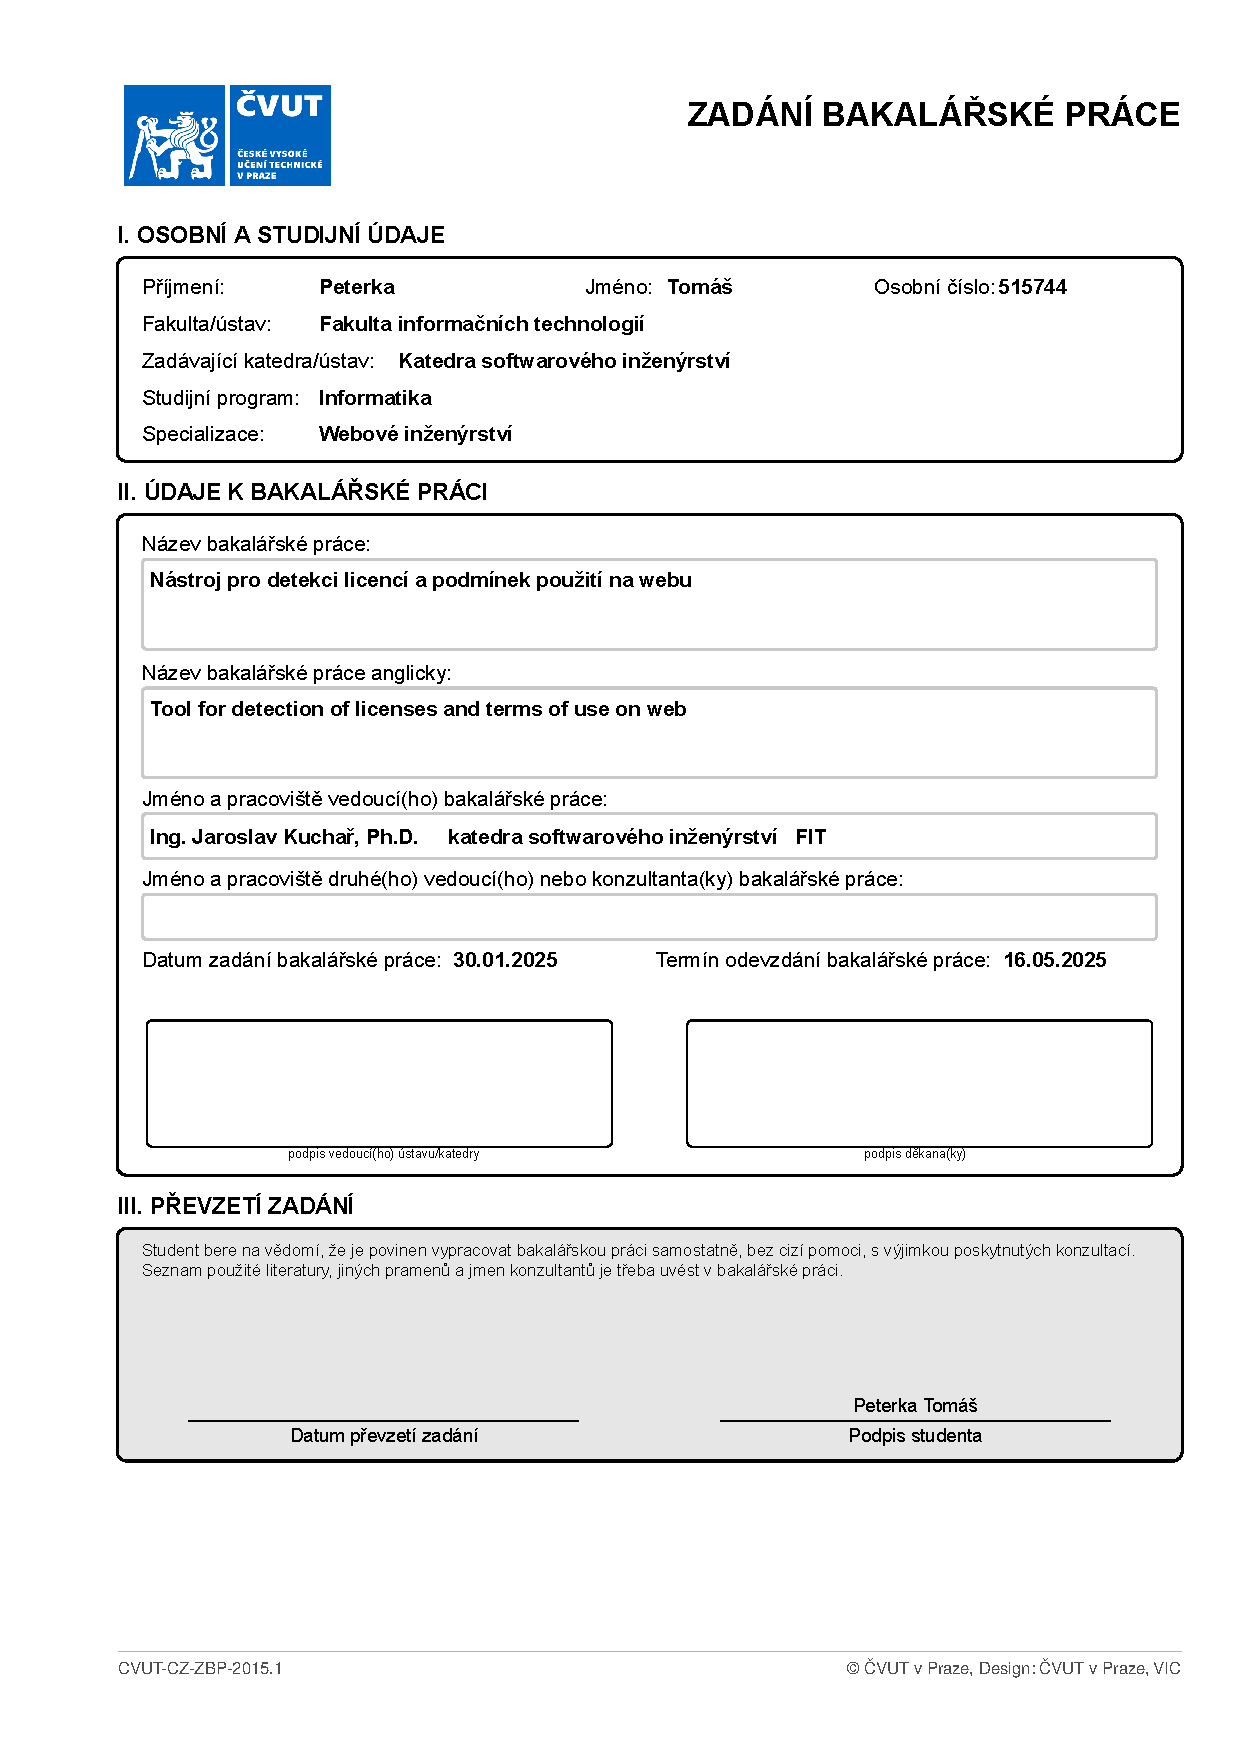
\includepdf[pages={1-}]{petert13-assignment.pdf} % replace this file with your thesis assignment generated from ProjectsFIT

\imprintpage % do not remove this command
\stopTOCentries
%%%%%%%%%%%%%%%%%%%%%%
% list of other contents END
%%%%%%%%%%%%%%%%%%%%%%

%%%%%%%%%%%%%%%%%%%
% ACKNOWLEDGMENT
% FILL IN / MODIFY
% This is a place to thank people for helping you. It is common to thank your supervisor.
%%%%%%%%%%%%%%%%%%%
\begin{acknowledgmentpage}
	Rád bych poděkoval vedoucímu mé bakalářské práce Ing. Jaroslavu Kuchařovi, Ph.D., za jeho odborné vedení, cenné rady, trpělivost a podporu během celé doby zpracování této práce.
    Velké poděkování patří také mé rodině za jejich trvalou podporu, povzbuzení a pochopení, které mi poskytovali po celou dobu studia i při realizaci této práce.
\end{acknowledgmentpage} 
%%%%%%%%%%%%%%%%%%%
% ACKNOWLEDGMENT END
%%%%%%%%%%%%%%%%%%%


%%%%%%%%%%%%%%%%%%%
% DECLARATION
% FILL IN / MODIFY
%%%%%%%%%%%%%%%%%%%
% INSTRUCTIONS
% ENG: choose one of approved texts of the declaration. DO NOT CREATE YOUR OWN. Find the approved texts at https://courses.fit.cvut.cz/SFE/download/index.html#_documents (document Declaration for FT in English)
% CZE/SLO: Vyberte jedno z fakultou schvalenych prohlaseni. NEVKLADEJTE VLASTNI TEXT. Schvalena prohlaseni najdete zde: https://courses.fit.cvut.cz/SZZ/dokumenty/index.html#_dokumenty (prohlášení do ZP)
\begin{declarationpage}
    Prohlašuji, že jsem předloženou práci vypracoval samostatně a že jsem uvedl veškeré použité
    informační zdroje v souladu s Metodickým pokynem o dodržování etických principů při přípravě
    vysokoškolských závěrečných prací.
    
    Beru na vědomí, že se na moji práci vztahují práva a povinnosti vyplývající ze zákona č. 121/2000 Sb.,
    autorského zákona, ve znění pozdějších předpisů, zejména skutečnost, že České vysoké učení
    technické v Praze má právo na uzavření licenční smlouvy o užití této práce jako školního díla podle §
    60 odst. 1 citovaného zákona.

    Prohlašuji, že jsem v průběhu příprav a psaní závěrečné práce použil nástroje umělé inteligence.
    Vygenerovaný obsah jsem ověřil. Stvrzuji, že jsem si vědom, že za obsah závěrečné práce plně zodpovídám.
\end{declarationpage}
%%%%%%%%%%%%%%%%%%%
% DECLARATION END
%%%%%%%%%%%%%%%%%%%

\printabstractpage % do not remove this command

%%%%%%%%%%%%%%%%%%%
% SUMMARY
% FILL IN / MODIFY
% OR REMOVE ENTIRELY (upon agreement with your supervisor)
% (appropriate to remove in most theses)
%%%%%%%%%%%%%%%%%%%
% \begin{summarypage}
% \section*{Summary section}
% 
% \lipsum[1][1-8]
% 
% \section*{Summary section}
% 
% \lipsum[2][1-6]
% 
% \section*{Summary section}
% 
% \lipsum[3]
% 
% \section*{Summary section}
% 
% \lipsum[2]
% 
% \section*{Summary section}
% 
% \lipsum[1][1-8] Lorem lorem lorem.
% \end{summarypage}
%%%%%%%%%%%%%%%%%%%
% SUMMARY END
%%%%%%%%%%%%%%%%%%%

\tableofcontents % do not remove this command
%%%%%%%%%%%%%%%%%%%%%%
% list of other contents: figures, tables, code listings, algorithms, etc.
% add/remove commands accordingly
%%%%%%%%%%%%%%%%%%%%%%
\listoffigures % list of figures
\begingroup
\let\clearpage\relax
\listoftables % list of tables
\thectufitlistingscommand
\endgroup

%%%%%%%%%%%%%%%%%%%
% ABBREVIATIONS
% FILL IN / MODIFY
% OR REMOVE ENTIRELY
% List the abbreviations in lexicography order.
%%%%%%%%%%%%%%%%%%%
\chapter{\thectufitabbreviationlabel}
	
\begin{tabular}{rl}
    AGPL & Affero General Public License \\
    AI & Artificial Intelligence \\
    API & Application Programming Interface \\
    BERT & Bidirectional Encoder Representations from Transformers \\
    BSD & Berkeley Software Distribution (License) \\
    CC & Creative Commons \\
    CSS & Cascading Style Sheets \\
    DOM & Document Object Model \\
    GPL & General Public License \\
    GPT & Generative Pre-trained Transformer \\
    HTML & HyperText Markup Language \\
    HTTP & HyperText Transfer Protocol \\
    JSON & JavaScript Object Notation \\
    LGPL & Lesser General Public License \\
    LLM & Large Language Model \\
    MIT & Massachusetts Institute of Technology (License) \\
    NLG & Natural Language Generation \\
    NLP & Natural Language Processing \\
    NLU & Natural Language Understanding \\
    POS & Part of Speech \\
    REST & Representational State Transfer \\
    ROGUE & Recall-Oriented Understudy for Gisting Evaluation \\
    SPDX & Software Package Data Exchange \\
    ToS & Terms of Service \\
    UA & User Agent \\
    URL & Uniform Resource Locator \\
\end{tabular}
%%%%%%%%%%%%%%%%%%%
% ABBREVIATIONS END
%%%%%%%%%%%%%%%%%%%
\resumeTOCentries
\mainmatter\mainmatterinit % do not remove these two commands
%%%%%%%%%%%%%%%%%%%
% THE THESIS
% MODIFY ANYTHING BELOW THIS LINE
%%%%%%%%%%%%%%%%%%%

% Do not forget to include Introduction
%---------------------------------------------------------------
%\chapter{Úvod}
% uncomment the following line to create an unnumbered chapter
\chapter*{Úvod}\addcontentsline{toc}{chapter}{Úvod}\markboth{Úvod}{Úvod}
%---------------------------------------------------------------

V dnešní době digitálních technologií je dostupnost webového obsahu obrovská a neustále roste.
S tím však přibývá i množství právních dokumentů, jako jsou licence a podmínky použití, které uživatelé často přehlížejí.
Přesto jsou tyto dokumenty klíčové, protože vymezují, jak mohou uživatelé obsah sdílet, upravovat a dále využívat.
Neznalost těchto podmínek může vést k neúmyslnému porušení autorských práv, což v některých případech může mít i právní důsledky.

Hlavním problémem je, že právní dokumenty jsou často dlouhé, složitě formulované a pro běžné uživatele obtížně srozumitelné.
To vede k tomu, že je uživatelé vnímají spíše jako obtíž a ignorují je, aby dosáhli svých cílů, aniž by byli omezováni \cite{Obar02012020}. 

Cílem této práce je analyzovat metody extrakce informací z webových zdrojů a navrhnout a implementovat nástroj, který pomocí těchto metod dokáže detekovat licence a zpracovat podmínky použití na webových stránkách.
Tento nástroj tak uživatelům poskytne stručné a relevantní informace o licenčních omezeních, čímž usnadní orientaci v textech o podmínkách použití obsahu.

Práce je rozdělena do čtyř hlavních kapitol, které postupně pokrývají analýzu, návrh, implementaci a testování nástroje.
V první kapitole jsou analyzovány licence a podmínky použití na webu, web scraping, jazykové modely, zpracování přirozeného jazyka a existující řešení.
Druhá kapitola se věnuje návrhu nástroje, včetně požadavků, architektury a prototypu webové aplikace.
Třetí část se zaměřuje na implementaci, zahrnující výběr technologií, extrakci a zpracování dat, využití jazykových modelů a vývoj prototypu.
A nakonec čtvrtá kapitola, která zahrnuje testování nástroje a hodnocení přesnosti jazykových modelů.

Téma této práce bylo vybráno z důvodu její vysoké aktuálnosti spojené s rozmachem využívání jazykových modelů.
Navíc současné principy zpracování přirozeného jazyka a rostoucí význam jazykových modelů nacházejí široké uplatnění i v řadě dalších oblastech.
\setcounter{page}{1}

%---------------------------------------------------------------
\chapter{Analýza}

\begin{chapterabstract}
    Před zahájením návrhu a implementace nástroje je nezbytné provést analýzu klíčových aspektů problému.
    Tato kapitola se věnuje rozboru licencí a podmínek použití na webových stránkách, technikám web scrapingu pro extrakci informací z webových zdrojů, principům fungování jazykových modelů, zpracování přirozeného jazyka a přehledu existujících nástrojů a řešení.
    Cílem je vytvořit pevný základ pro další fáze vývoje nástroje.
\end{chapterabstract}

\section{Licence na webu}
Licence na webu představují rámec, který definuje, jak mohou uživatelé nakládat s obsahem dostupným na internetu.
Tyto licence jsou klíčovým prvkem pro ochranu duševního vlastnictví a zároveň umožňují stanovit jasná pravidla pro další využití obsahu.
Existuje více než 400 různých licencí, které se liší podle toho, jaké podmínky stanovují. Každá taková licence může být využívána pro různé druhy obsahu, jako jsou texty, obrázky, videa nebo software.
Každá licence má navíc své vlastní zkratky či symboly, které ji identifikují. \cite{spdxSPDXLicense}

Licence na webu lze rozdělit do několika základních kategorií podle toho, jaké podmínky stanovují pro využívání obsahu: 
\begin{description}
    \item[Proprietární licence:] Tyto licence jsou nejrestriktivnější a znemožňují kopírování, úpravy nebo distribuci obsahu. Chrání tak vlastníka před neoprávněným použitím.
    \item[Public domain:] Obsah označený jako public domain je volně dostupný k použití a úpravám bez jakýchkoli omezení.
    \item[Unlicensed:] Pokud není explicitně uvedena licence, obsah podléhá autorskému právu a jeho použití může být omezeno, i když podmínky nejsou jasně specifikovány.
    \item[Open source licence:] Umožňují používání, úpravy a sdílení obsahu za určitých podmínek. Dělí se na následující kategorie:
        \begin{description}
            \item[Permisivní licence:] (např. Apache, MIT, BSD) Jedná se o licence, které zajišťují velmi volné použití softwaru. Umožňují jeho začlenění do komerčních i soukromých projektů, přičemž se liší například v požadavcích na zachování licenčních upozornění nebo autorských práv.
            \item[Copyleft licence:] (např. GPL, AGPL) Tyto restriktivní licence vyžadují, aby upravený nebo distribuovaný software byl šířen pod stejnou licencí.
            \item[GNU/LGPL:] Umožňuje vývojářům propojit svůj software s otevřenými knihovnami a licencovat výsledný kód podle vlastního uvážení, včetně proprietárních licencí. Podmínkou však je, že samotná knihovna musí zůstat pod licencí LGPL  \cite{snykOpenSource}
        \end{description}
\end{description} 

Zatímco většina open source licencí nachází uplatnění především v oblasti softwaru, pro obsah na webových stránkách, jako jsou texty, obrázky či multimédia, existují otevřené licence typu Creative Commons.
Ty se staly standardem mezi otevřenými licencemi díky své flexibilitě a přizpůsobivosti různým typům tvůrčího obsahu.
V současnosti je evidována více než jedna miliarda využití \cite{libguidesGuidesUsing}, což svědčí o jejich širokém přijetí.

\subsection{Creative Commons}
Creative Commons (CC) je mezinárodní nezisková organizace, která podporuje rozšiřování a udržování společného prostoru sdílených znalostí a kultury. 
Creative Commons licence poskytují standardizovaný způsob, jak mohou jednotliví tvůrci i velké korporace povolit veřejnosti využívat jejich autorská díla v souladu s autorským právem.
Z pohledu uživatele, který dílo znovu používá, existence Creative Commons licence na chráněném díle objasňuje, co s tímto dílem může dělat. \cite{creativecommonsAboutLicenses}

Existuje šest základních typů CC licencí, které se liší v podmínkách použití:
\begin{description}
    \item[CC BY:] Nejotevřenější licence, která umožňuje redistribuci, vytváření odvozenin a dokonce komerční využití díla za podmínky, že je uveden původní autor a jsou označeny případné změny.
    \item[CC BY-SA:] Podobná jako CC BY, ale vyžaduje, aby odvozená díla byla sdílena pod stejnou licencí.
    \item[CC BY-NC:] Povoluje sdílení a úpravy díla, ale pouze pro nekomerční účely.
    \item[CC BY-ND:] Umožňuje redistribuci díla, ale zakazuje jeho úpravy.
    \item[CC BY-NC-SA:] Kombinuje podmínky nekomerčního využití a sdílení pod stejnou licencí.
    \item[CC BY-NC-ND:] Nejrestriktivnější CC licence, která povoluje pouze sdílení původního díla pro nekomerční účely bez možnosti úprav. \cite{creativecommonsAboutLicenses}
\end{description}
Speciálním případem je licence CC0, která umožňuje autorům uvolnit své dílo do veřejného vlastnictví a zříci se všech autorských práv.
Tato licence tak spadá do kategorie „Public domain“ a je určena pro autory, kteří chtějí, aby jejich dílo bylo volně dostupné bez jakýchkoli podmínek.

Reprezentace takových licencí by pak měla být jednoznačná a snadno identifikovatelná, aby uživatelé mohli rychle zjistit, jak mohou daný obsah využívat.
Doporučeným způsobem, jak licenci zobrazit, je uvést stručný text s informací o licenci a odkazem na vybranou CC licenci, například: \textit{© 2019. This work is openly licensed via} \href{https://creativecommons.org/licenses/by/4.0/}{CC BY 4.0}.
Pro pokročilejší zobrazení lze využít HTML kód přímo od CC. \cite{creativecommonsAboutLicenses}

Umístění označení licence na webových stránkách není nijak standardizované a může se lišit na základě konkrétního obsahu.
Pokud se jedná o konkrétní média jako obrázky nebo videa, bývá licence často zobrazena přímo u obsahu.
Ale pokud se jedná o celou webovou stránku, bývá licence zobrazena v patičce stránky nebo je zmíněna v rámci textu podmínek použití.
Tato pozorování byla získána během analýzy několika desítek webových stránek, obsahujících různé typy CC licencí.

\section{Podmínky použití na webu}
Dalším, již dříve zmíněným, způsobem jak omezit využití obsahu na webových stránkách, jsou podmínky použití.
Podmínky použití (ToS) stanovují pravidla, která musí jednotlivci nebo organizace dodržovat, aby mohli platformu využívat.
Tyto podmínky jsou obvykle právně závazné, pokud neporušují místní zákony.
Poskytovatel může tyto podmínky čas od času upravit a je jeho povinností informovat uživatele o jakýchkoli změnách. \cite{pcmagDefinitionTerms}

Na rozdíl od licencí, které se primárně zaměřují na autorská práva a způsoby využití obsahu, ToS pokrývají širší spektrum aspektů souvisejících s používáním webových stránek.
Zavedení ToS přináší provozovatelům webů řadu důležitých výhod.
Vymezují pravidla, která musí uživatelé dodržovat při využívání služeb, čímž pomáhají omezit zneužívání webu.
Zároveň slouží k omezení právní odpovědnosti provozovatele a snižují tak potenciální rizika.
Navíc mohou objasnit, komu patří obsah na webu, a stanovují tak vlastnická práva.

Reprezentace těchto podmínek není striktně standardizovaná a může se na různých webových stránkách lišit.
Avšak je v zájmu autorů, aby byly ToS snadno rozpoznatelné, což vytváří často používané textové vzory jak podmínky zobrazit.

\clearpage
Analyzováno bylo více než sto webových stránek (v anglickém jazyce).
Tento vzorek je tvořen jednak stránkami, které byly nalezeny při rešerši k tématu práce, a jednak výběrem z nejnavštěvovanějších webů dle \cite{dataforseo1000Websites}.
Na základě této analýzy byly identifikovány následující časté textové vzory odkazující na ToS nebo jejich části:\begin{itemize}
    \item \textit{Terms of Service}
    \item \textit{Terms and Conditions}
    \item \textit{Terms of Use}
    \item \textit{License}
    \item \textit{Legal}
\end{itemize}

Aby uživatelé mohli snadno zjistit, jak mohou obsah využívat, je důležité, aby byly ToS snadno dostupné.
Podobně jako u licencí, nelze určit jejich jednoznačné umístění na webových stránkách.
Nicméně při analýze stránek bylo zjištěno, že patička webových stránek je nejčastějším místem, kde jsou ToS umístěny.

Patička totiž obvykle zahrnuje informace týkající se své sekce, jako jsou odkazy na související dokumenty, údaje o autorských právech či autora patičky.
Pokud patička obsahuje rozsáhlé části obsahu, tyto části obvykle představují přílohy, rejstříky, podrobné licenční smlouvy nebo jiný podobný obsah \cite{w3449Footer}.
Z tohoto důvodu není překvapující, že vzory textů ToS i označení licencí byly v rámci analýzy nejčastěji identifikovány právě v patičce.

\section{Web scraping}
Aby bylo možné získat informace o licencích a podmínkách použití na webových stránkách, je nutné provést extrakci dat.
Aby tato extrakce nemusela být prováděna ručně, což by bylo velmi pracné a náročné, využívá se automatizovaná technika známá jako web scraping.

Web scraping je proces, který získává nestrukturovaná data, jako je HTML obsah webových stránek, a převádí je do strukturovaných formátů, což usnadňuje jejich analýzu či ukládání.
Tato technika je zvláště důležitá v situacích, kdy by ruční sběr dat byl nepraktický kvůli rozsahu nebo četnosti aktualizací, například při sledování tržních trendů v reálném čase nebo shromažďování výzkumných datových sad.
Tím, že umožňuje přístup k jinak pracně získatelným informacím, web scraping slouží jako výkonný nástroj napříč průmyslovými odvětvími i akademickou sférou. \cite{inbook}

Metody a nástroje používané při web scrapingu se přizpůsobují různým technickým potřebám a složitostem webových stránek. Mezi využívané techniky patří přístupy, jako je porovnávání textových vzorů pomocí regulárních výrazů, ale i pokročilejší metody, například parsování DOM, které cílí na konkrétní prvky webové stránky.
Používají se také automatizační nástroje simulující lidské prohlížení, které umožňují zpracování dynamického obsahu generovaného JavaScriptem. \cite{inbook}
Tyto možnosti tak umožňují přizpůsobit web scraping dle potřeb použití, ať už jde o jednoduchou extrakci dat, nebo složité webové struktury.

Navzdory své užitečnosti čelí web scraping mnoha výzvám, které jeho použití komplikují.
Právní a etické otázky představují hlavní překážky, protože web scraping může být v rozporu s podmínkami používání webových stránek nebo zákony o duševním vlastnictví, což vytváří nejasné prostředí pro jeho využití.
Kromě toho technické bariéry, jako jsou CAPTCHA, blokování IP adres nebo neustále se měnící rozložení stránek, vyžadují neustálé inovace, aby scraping zůstal efektivní.
Kvalita získaných dat také představuje problém, protože nekonzistence nebo neúplné informace často vyžadují další zpracování. \cite{inbook}

Při web scrapingu je tak důležité dodržovat etické standardy.
Mnoho webových stránek zakazuje procházení svého obsahu vyhledávacími roboty (využívající web scraping) pomocí souboru \textit{robots.txt}.
Tento soubor je obvykle umístěn v kořenovém adresáři webové stránky (například \url{https://www.example.com/robots.txt}) a určuje, zda mohou vyhledávací roboti přistupovat k celému webu nebo jen k vybraným zdrojům \cite{mozillaRobotstxtDocs}.
Ačkoli tento soubor nezastaví nikoho, kdo chce web scraping provádět, je etickým standardem jej respektovat.

\section{NLP}
Zpracování přirozeného jazyka (NLP) je disciplína na pomezí umělé inteligence a počítačové lingvistiky, jejímž cílem je umožnit počítačům porozumět, interpretovat a generovat lidský jazyk.
NLP lze rozdělit do dvou hlavních oblastí:
\begin{enumerate}
    \item \textbf{Generování přirozeného jazyka (NLG)} 
    \item \textbf{Porozumění přirozenému jazyku (NLU)} 
\end{enumerate}
Mezi procesy spojené s chápáním a tvorbou textového obsahu, které tyto kategorie zahrnují, patří mimo jiné:
\begin{itemize}  
    \item \textbf{Rozpoznávání pojmenovaných entit} \\
    Identifikace a klasifikace entit v textu. \\
    \textit{Příklady entit:} osoby, organizace, místa, data.
    
    \item \textbf{Strojový překlad} \\
    Automatický převod textu z jednoho jazyka do druhého.
    
    \item \textbf{Odpovídání na otázky} \\
    Automatické vyhledávání a poskytování odpovědí na otázky položené v přirozeném jazyce.
    
    \item \textbf{Analýza sentimentu} \\
    Určení emocí nebo postoje vyjádřeného v textu a jeho klasifikace jako: pozitivní, negativní, neutrální.
    
    \item \textbf{Generování textu} \\
    Tvorba textu podobného lidskému na základě zadaných podmínek nebo podnětů.
    
    \item \textbf{Označování slovních druhů (POS tagging)} \\
    Přiřazení každému slovu ve větě konkrétního slovního druhu. \cite{Kondurkar2023} \\
\end{itemize}

NLP se neustále vyvíjí díky pokrokům v hlubokém učení, dostupnosti rozsáhlých datových sad a rostoucí poptávce po inteligentních systémech pro zpracování jazyka.
Klíčovou roli v tomto vývoji hrají moderní jazykové modely, které významně posouvají možnosti NLP.

\subsection{Jazykové modely}
Jazykové modely existují již od 80. let 20. století a slouží ke statistickému modelování vlastností přirozeného jazyka na základě analýzy textů, například frekvencí slov, jejich pravděpodobností a kontextu.
Díky nedávnému nárůstu dostupnosti textových sbírek a zlepšení výpočetních zdrojů byly představeny velké jazykové modely (LLM), které přinesly revoluci do pole NLP.
LLM vycházejí ze stejných principů jako tradiční jazykové modely, ale díky obrovským textovým databázím, často zahrnujícím téměř celý web, je možné trénovat mnohem větší a výkonnější modely. \cite{10.3389/frai.2023.1350306}

V rámci NLP přinesly zásadní změnu zejména modely hlubokého učení, konkrétně architektury typu transformer, jako jsou BERT (Bidirectional Encoder Representations from Transformers) nebo GPT (Generative Pre-trained Transformer).
Tyto modely výrazně posílily schopnosti systémů porozumět a generovat jazyk podobný lidskému.
Díky nim se zlepšily výsledky v úlohách jako strojový překlad, vývoj chatbotů, analýza sentimentu a dalších jazykových aplikací.
Transformátorové modely využívají trénink na rozsáhlých datových sadách, což jim umožňuje zachytit nuance jazyka a efektivně zpracovávat složité textové struktury. \cite{SureshBabu2023}

V dnešní době existuje celá řada modelů a to jak open source, tak proprietárních.
Navíc čím dál častěji vznikají nové modely, které dosahují stále lepších výsledků.
To však ztěžuje jednoznačné určení dlouhodobě nejlepšího modelu pro konkrétní účel.
Dne 6. 4. 2025 je na prvních příčkách model \textit{Gemini-2.5-Pro-Exp}. \cite{lmarenaAI, trackingaiTracking}

K detekci licencí lze tak využít základní metody NLP, jako například rozpoznávání pojmenovaných entit, které dokáže identifikovat klíčové informace v textu a přiřadit jim konkrétní kategorie.
Avšak pro zpracování složitějších textů, jako jsou ToS, se jako vhodnější jeví moderní jazykové modely, které díky svému tréninku na rozsáhlých datových sadách a schopnosti zachytit kontext a nuance jazyka, umožňují hlubší analýzu textu.

\section{Existující nástroje a řešení}
V oblasti detekce a analýzy licenčních podmínek existuje několik nástrojů a řešení.
Mezi ně například patří FOSSA \cite{fossaFOSSAControl}, FOSSID \cite{fossID}, Black Duck \cite{blackduckApplicationSecurity} či FOSSology \cite{fossologyFOSSology}.
Avšak všechny tyto nástroje se zaměřují především na detekci open source licencí v kódu.
V rámci této analýzy tedy nebyl nalezen volně využívaný nástroj, který by řešil detekci licencí a zpracování podmínek použití na webových stránkách.

Avšak byla nalezena bakalářská práce \cite{essay100804}, která se zabývá tématem \textit{License-aware web crawling}.
V práci je popsán vývoj nástroje, který využívá web scraping k extrakci licenčních informací z webových stránek.
Na základě těchto informací je za pomocí NLP technik detekována CC licence a je zobrazena extrahovaná část ToS textu.
Práce byla zhotovena v rámci projektu LAW4OSAI (License-Aware Web Crawling for Open Search AI), který má za cíl propojit právní expertizu s technologickými pokroky ve vyhledávání na webu.
Prostřednictvím licencovaného procházení webového obsahu chce projekt podpořit transparentnější a právně souladný přístup k vyhledávání \cite{openwebsearchProjectLAW4OSAI}. 
Ačkoli řešení této práce nikterak nevyužívá jazykové modely a dále nezpracovává získaný ToS text, tak stále může posloužit jako inspirace pro návrh a implementaci nástroje v rámci této práce.

\section{Shrnutí}
Na základě analýzy dílčích témat bylo identifikováno několik poznatků, které budou dále využity při návrhu a implementaci nástroje.
Bylo zjištěno, že licence a ToS na webových stránkách jsou klíčovými dokumenty, které definují pravidla pro využití obsahu.
Nejčastěji využívané licence na webových stránkách jsou Creative Commons, které umožňují autorům jednoduše definovat podmínky pro využití obsahu.
Zároveň bylo zjištěno, že reprezentace těchto dokumentů není standardizovaná a může se lišit na základě konkrétního obsahu.
Nicméně byly identifikovány časté textové vzory, které se používají pro zobrazení licencí a ToS na webových stránkách.
Také bylo zjištěno, že společné umístění těchto dokumentů se nachází zpravidla v patičce webových stránek.
Pro extrakci informací z webových stránek byl analyzován web scraping, který umožňuje získat strukturovaná data z nestrukturovaných nebo polostrukturovaných dat.
Následně pro zpracování získaných dat byly prozkoumány jazykové modely, které umožňují analýzu textu a porozumění jeho kontextu.
Nakonec byly identifikovány existující nástroje a řešení, ze kterých jako nejpřínosnější byla vybrána bakalářská práce \cite{essay100804}, která se zabývá tématem \textit{License-aware web crawling}.
%---------------------------------------------------------------

\chapter{Návrh}

\begin{chapterabstract}
    Kapitola popisuje návrh nástroje pro analýzu CC licencí a ToS na webových stránkách.
    Definuje funkční a nefunkční požadavky, navrhuje architekturu s procesy extrakce a zpracování dat a představuje prototyp webové aplikace s API a uživatelským rozhraním.
\end{chapterabstract}

\section{Požadavky na nástroj}
Požadavky na nástroj představují základ jeho návrhu a následné implementace, jelikož definují očekávané chování a vlastnosti systému.
Požadavky v této práci vycházejí z potřeby automatizovat analýzu CC licencí a ToS na webových stránkách, což je úkol, který vyžaduje efektivní zpracování dat a jejich srozumitelnou prezentaci uživateli.
V rámci návrhu jsou tak požadavky rozděleny do dvou kategorií: funkční a nefunkční.
Funkční požadavky specifikují konkrétní funkcionality, které nástroj musí nabízet, aby splnil svůj účel, jako je detekce licencí nebo analýza textů pomocí jazykových modelů.
Naopak nefunkční požadavky se zaměřují na kvalitativní aspekty nástroje, včetně jeho výkonu, spolehlivosti a uživatelské přívětivosti.

\subsection{Funkční požadavky}
\label{chap:functional}
\begin{description}
    \item[Detekce CC licence:] Detekce použitých Creative Commons licencí na webových stránkách.
    \item[Klasifikace licence:] Rozpoznání konkrétního typu CC licence.
    \item[Detekce ToS odkazů:] Identifikace klíčových textových vzorů vedoucích k ToS textu.
    \item[Zpracování ToS textu:] Analýza extrahovaného ToS textu pomocí jazykových modelů.
    \item[Vizualizace výsledků:] Vizualizace detekovaných licencí a zpracovaných podmínek použití ve webovém rozhraní.
    \item[API:] Možnost přístupu k funkcím nástroje pomocí API, které by mělo být navrženo s REST API principy.
\end{description}

\subsection{Nefunkční požadavky}
\label{chap:nonfunctional}
\begin{description}
    \item[Výkon:] Nástroj by měl za standardních podmínek detekovat ToS text a CC licenci na webové stránce do 5 sekund.
    \item[Spolehlivost:] Detekce licencí a ToS odkazů by měla dosahovat přesnosti alespoň 90\%.
    \item[Přívětivost:] Nástroj by měl být intuitivní a snadno použitelný.
\end{description}

\section{Architektura nástroje}
Nástroj pro detekci licencí a podmínek použití na webu je navržen jako knihovna, která poskytuje funkcionality pro extrakci a analýzu dat z webových stránek.
Tato knihovna je nezávislou komponentou, která může být využita v různých kontextech, jako jsou skripty automatizovaných procesů nebo webové aplikace.
Hlavním cílem tohoto návrhu je zajistit flexibilitu a znovupoužitelnost, aby nástroj mohl být snadno integrován do různých prostředí bez nutnosti dalších nadstaveb.
Obecný návrh architektury nástroje je znázorněn na obrázku \ref{fig:architecture}.

\subsection{Knihovna}
Proces návrhu knihovny je rozdělen do dvou hlavních částí, aby bylo možné efektivně využít jazykové modely při zpracování textů ToS.
První část se zaměřuje na základní analýzu a extrakci dat z webových stránek s cílem získat co nejvíce relevantních informací.
Druhá část zahrnuje využití jazykových modelů, které provádějí hlubší analýzu extrahovaných textů, jako je sumarizace nebo odpovídání na dotaz.
Toto rozdělení umožňuje uživateli získat data z webových stránek ještě před tím, než jsou zpracována jazykovými modely.
Díky tomu je možné nástroj využít i bez použití jazykových modelů, což může být užitečné v případech, kdy uživatelé nechtějí nebo nemohou využívat API jazykových modelů.

Navržená knihovna je založena na modulární architektuře, která zajišťuje rozdělení funkcionalit do samostatných komponent.
Každá komponenta je zodpovědná za konkrétní část zpracování dat, což umožňuje snadnou rozšiřitelnost.
Jak lze vidět na obrázku \ref{fig:architecture}, knihovna se skládá z následujících komponent:
\begin{description}
    \item[Modul pro správu požadavků:] Zajišťuje komunikaci s webovými servery, včetně načítání stránek a ověřování přístupu podle pravidel definovaných v souboru robots.txt. Slouží jako vstupní bod pro získávání dat z webových zdrojů.
    \item[Modul pro extrakci dat:] Zodpovědný za parsování HTML obsahu stránek a získání relevantních informací.
    \item[Modul identifikace licence:] Provádí analýzu textu a odkazů za účelem identifikace konkrétních typů licencí, na základě předdefinovaných vzorů a klíčových slov.
    \item[Modul zpracování ToS:] Oddělený modul, který zpracovává vyfiltrovaný ToS text pomocí jazykových modelů.
\end{description}

\begin{figure}[H]
    \centering
    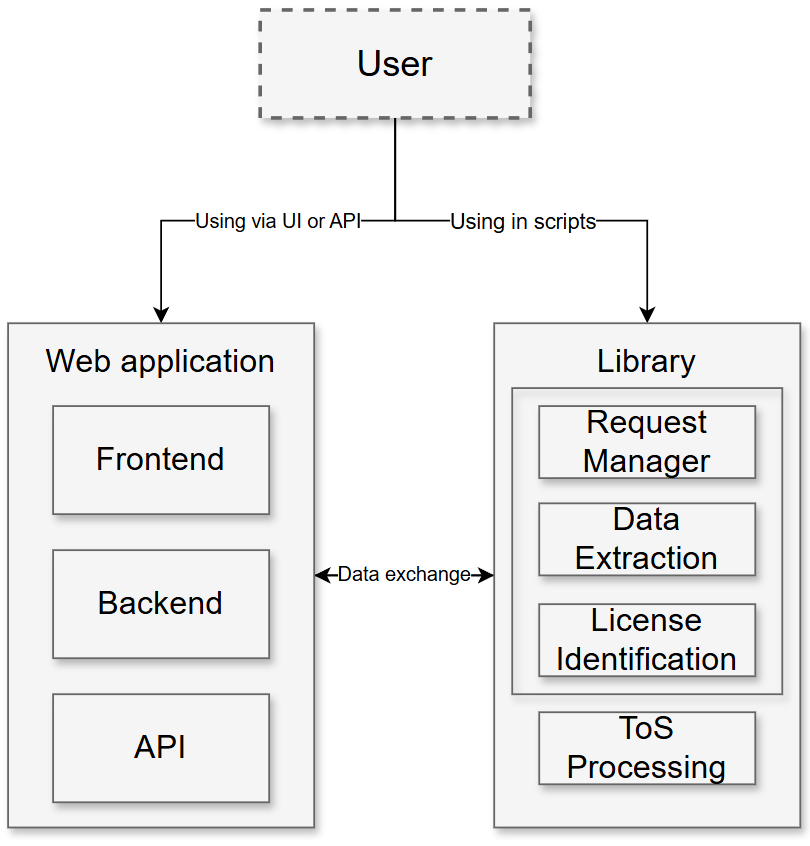
\includegraphics[width=\linewidth]{images/architecture}
    \caption{Architektura nástroje}
    \label{fig:architecture}
\end{figure}

\subsubsection{Tok dat}
V rámci návrhu je důležité definovat, jakým způsobem budou jednotlivé komponenty spolupracovat a jakým způsobem budou data předávána mezi nimi.
Pro tento účel byly navrženy vývojové diagramy.
Tyto diagramy představují nástroj pro vizualizaci a popis procesů navrženého nástroje.
Umožňují tak přehledně znázornit tok dat a jednotlivé kroky zpracování, což usnadňuje pochopení návrhu nástroje.

První vývojový diagram \ref{fig:flowchart1} znázorňuje proces základní analýzy a extrakce dat z webových stránek, což tvoří první hlavní část navrženého nástroje.
Proces začíná zadáním URL adresy webové stránky, která má být analyzována.
Následně systém ověří, zda je zadaný odkaz platný, a pokud není, proces se ukončí s informací o neplatnosti odkazu.
V případě platného odkazu nástroj zkontroluje soubor robots.txt, aby zjistil, zda je web scraping obsahu povolen pro daného UA (User Agent).
Pokud povolen není, proces se ukončí s informací o nepovoleném přístupu.
V opačném případě nástroj provede web scraping stránky a pokračuje dvěma paralelními větvemi.
V první větvi hledá Creative Commons licenci a pokud ji nalezne, identifikuje její typ, a tuto informaci vrátí jako součást výsledků.
Pokud licenci nenalezne, vrátí odpovídající informaci.
Ve druhé větvi nástroj vyhledává odkazy na ToS text.
Pokud odkazy nejsou nalezeny, proces vrátí informaci o jejich nenalezení. V opačném případě nástroj z nalezených odkazů ToS text extrahuje a tento text filtruje, aby odstranil irelevantní části.
Nakonec jsou vráceny všechny dosud získané informace, které mohou zahrnovat typ licence, extrahovaný ToS text nebo důvod selhání, pokud některý krok neproběhl úspěšně.

\begin{figure}[H]
    \centering
    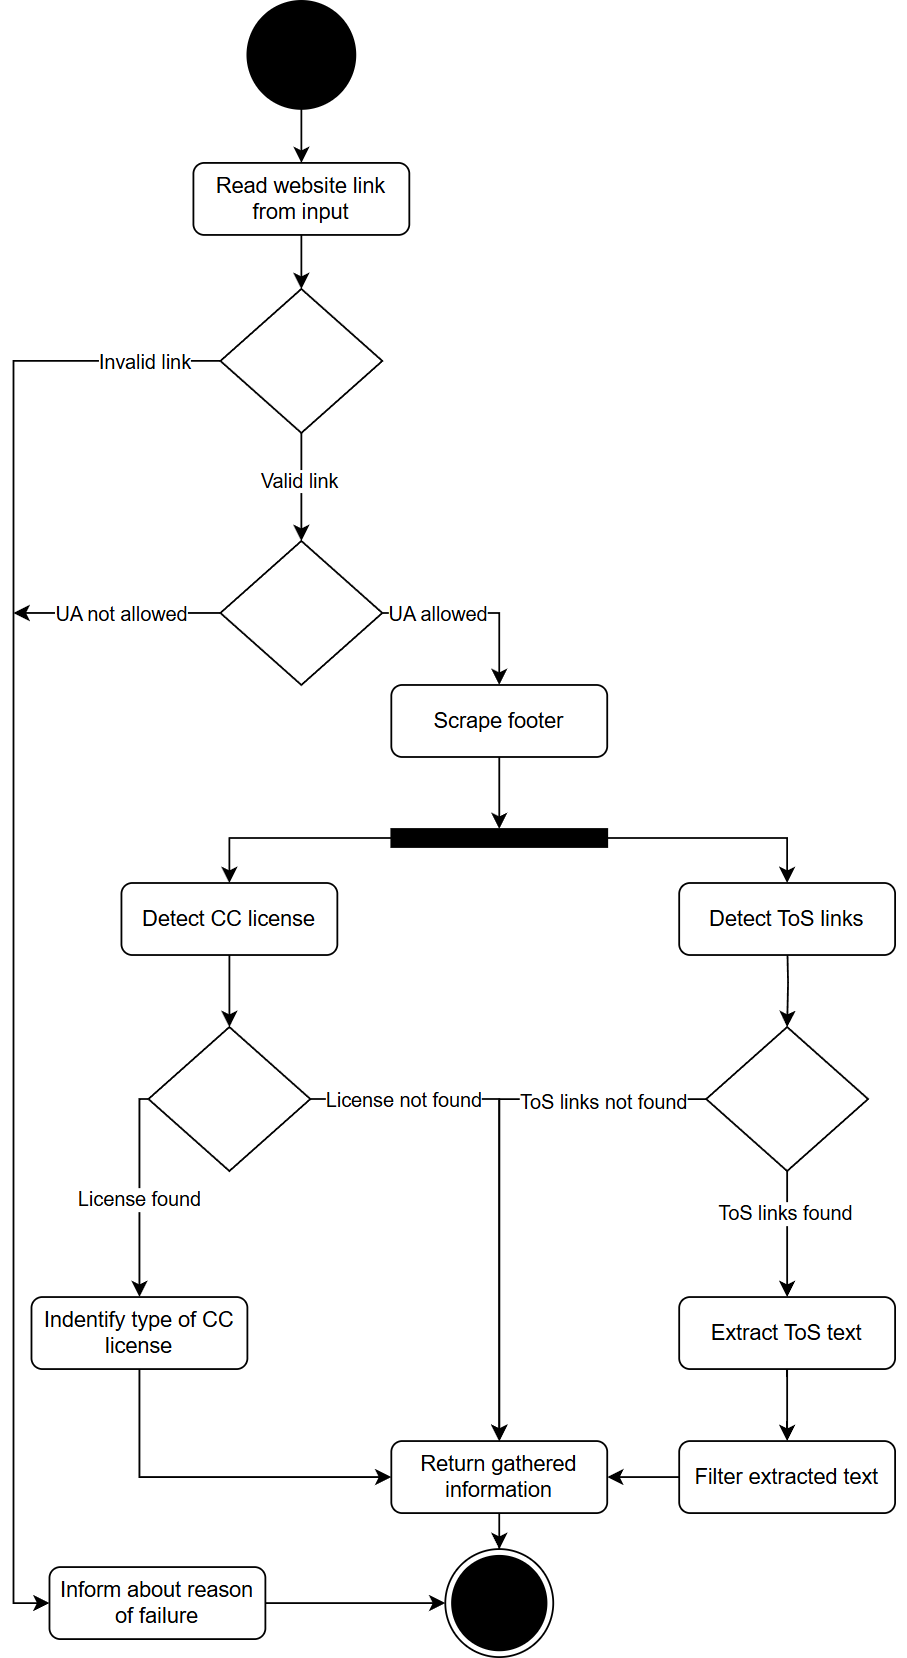
\includegraphics[width=0.8\linewidth]{images/flowchart1}
    \caption{Vývojový diagram 1. části nástroje}
    \label{fig:flowchart1}
\end{figure}

\clearpage
Druhý vývojový diagram \ref{fig:flowchart2} popisuje proces analýzy extrahovaných textů pomocí jazykových modelů, což představuje druhou hlavní část nástroje.
Proces začíná nastavením rozhraní API pro komunikaci s jazykovým modelem, který bude použit pro analýzu.
Následně uživatel volí jednu ze dvou hlavních akcí.
První možností je sumarizace textu, kdy jazykový model zpracuje vstupní text a vrátí jeho stručné shrnutí.
Druhou možností je odpověď na dotaz, kdy uživatel zadá otázku týkající se vstupního textu a jazykový model vrátí vygenerovanou odpověď.
Výsledkem procesu je tedy buď shrnutí textu, nebo odpověď na zadanou otázku, v závislosti na zvolené akci.


\begin{figure}[!htbp]
    \centering
    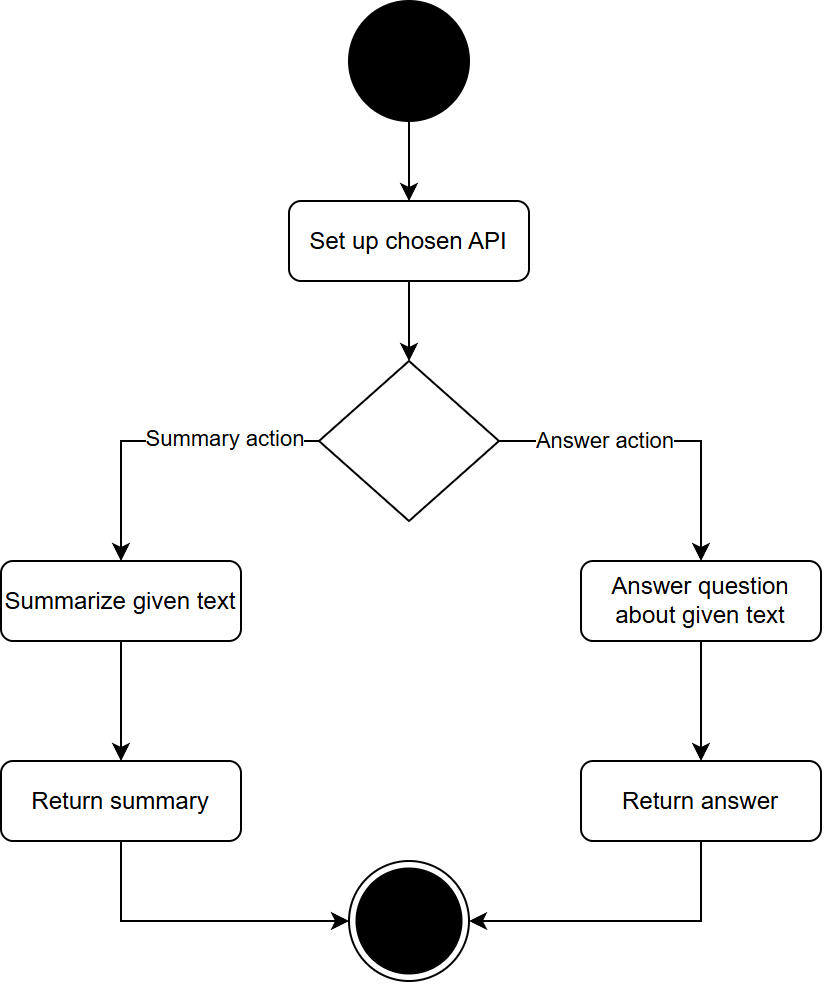
\includegraphics[width=0.8\linewidth]{images/flowchart2}
    \caption{Vývojový diagram 2. části nástroje}
    \label{fig:flowchart2}
\end{figure}

\clearpage

\subsection{Prototyp webové aplikace}
V průběhu tvorby zadání této bakalářské práce bylo s vedoucím práce rozhodováno o různých způsobech, jak nástroj používat.
Mimo využití nástroje, jakožto samostatné knihovny, bylo rozhodnuto o vytvoření prototypu webové aplikace, která by umožnila uživatelům snadno přistupovat k funkcím nástroje nejen prostřednictvím uživatelského rozhraní, ale také pomocí API.
Cílem tak není navrhnout plnohodnotnou webovou aplikaci obsahující plnohodnotnou databázi, uživatelské účty a další běžné části webových aplikací, ale spíše jednoduchý prototyp, který demonstruje funkčnost navrženého nástroje.

\subsubsection{Backend}
Backend webové aplikace je navržen jako centrální komponenta prototypu, která zprostředkovává zpracování požadavků od uživatele a koordinuje analýzu dat souvisejících s ToS a licencemi webových stránek.
Jeho hlavním cílem je zajistit propojení mezi uživatelským rozhraním a navrženou knihovnou. Součástí backendu je také API, které umožňuje externí přístup k funkcím nástroje.
Architektura backendu je navržena jako modulární systém:
\begin{description}
    \item[Router:] Komponenta odpovědná za směrování požadavků od uživatele a jejich předání příslušným službám. Definuje cesty pro interakci s uživatelem, například zadání URL adres nebo žádosti o pokročilou analýzu jazykovými modely.
    \item[Services:] Služby, které zajišťují koordinaci mezi routerem, API a analytickým nástrojem. Tyto služby zpracovávají požadavky, předávají data ke zpracování a vracejí výsledky ve formátu vhodném pro obě rozhraní.
    \item[API:] Programové rozhraní, které umožňuje externí přístup k funkcím nástroje. API je navrženo tak, aby zrcadlilo hlavní funkce systému a poskytovalo strukturované odpovědi pro analýzu, sumarizaci a odpovídání na otázky, čímž doplňuje interakci přes frontend.
\end{description}

Tok dat v backendu začíná přijetím požadavku z uživatelského rozhraní či API prostřednictvím routeru.
Router předá požadavek službám, které komunikují s knihovnou pro provedení analýzy webových stránek.
Výsledky jsou poté zpracovány a vráceny ve strukturované podobě a to buď frontendu pro zobrazení, nebo klientovi přes API.
Tento návrh zajišťuje oddělení prezentační a analytické vrstvy a díky integraci API rozšiřuje možnosti využití systému.

\clearpage
\subsubsection{API}
Navržené API má za cíl poskytnout alternativní rozhraní pro přístup k funkcím nástroje prostřednictvím HTTP požadavků, což umožňuje jeho využití bez nutnosti interakce přes uživatelské rozhraní.
API je určeno pro externí aplikace, skripty nebo automatizované procesy.
Je navrženo jako REST API, protože tento typ rozhraní je jednoduchý, široce používaný a vhodný pro komunikaci s různými typy klientů.
Při komunikaci jsou vstupní i výstupní data ve formátu JSON, což zajišťuje snadné zpracování dat na straně klienta.

Všechny operace jsou navrženy jako asynchronní, aby bylo možné efektivně zvládat časově náročné úkoly, jako je web scraping a generování textů pomocí jazykových modelů.
Každý endpoint používá HTTP metodu POST pro spuštění úlohy.
Po inicializaci úkolu vrací identifikátor úlohy a odkaz na další endpoint, který využívá metodu GET.
Tento doplňkový endpoint slouží k monitorování stavu úlohy a poskytuje přístup k výsledkům.
Všechny dílčí endpointy jsou popsané v tabulce \ref{tab:api_endpoints}.

Pro analýzu webových stránek slouží endpoint /scans, který zpracovává JSON požadavek se seznamem URL adres.
Výsledky, včetně informací o nalezených licencích a extrahovaných textech ToS, jsou dostupné přes doplňkový endpoint /scans/<task_id>.

Sumarizaci extrahovaných textů ToS zajišťuje endpoint /summaries.
Tento endpoint přijímá JSON požadavek s textem k sumarizaci a specifikací API rozhraní včetně příslušného API klíče.
Shrnutý text lze získat prostřednictvím /summaries/<task_id>.

K zodpovídání otázek týkajících se sumarizovaného textu je navržen endpoint /answers.
Přijímá JSON požadavek obsahující otázku, sumarizovaný text a specifikaci API rozhraní s API klíčem.
Odpověď je poskytována přes /answers/<task_id>.

\begin{table}[H]
	\centering
	\begin{tabular}{|p{0.35\textwidth}|p{0.15\textwidth}|p{0.4\textwidth}|}
		\hline
		\textbf{Endpoint} & \textbf{Metoda} & \textbf{Popis} \\ \hline
		/scans & POST & Analýza webových stránek \\ \hline
        \parbox{0.4\textwidth}{/scans/<task\_id>} & GET & Kontrola stavu analýzy a její vyzvednutí \\ \hline
		\parbox{0.4\textwidth}{/summaries} & POST & Sumarizace textu \\ \hline
		\parbox{0.4\textwidth}{/summaries/<task\_id>} & GET & Kontrola stavu sumarizace a její vyzvednutí \\ \hline
		/answers & POST & Odpověď na otázku \\ \hline
		\parbox{0.4\textwidth}{/answers/<task\_id>} & GET & Kontrola stavu odpovědi a její vyzvednutí \\ \hline
	\end{tabular}
	\caption{Přehled endpointů navrženého API}
	\label{tab:api_endpoints}
\end{table}

\clearpage
\subsubsection{Frontend}

Frontend je navržen jako uživatelské rozhraní prototypu, jehož účelem je umožnit interakci s backend částí a prezentovat dílčí výsledky nástroje.
Hlavním cílem frontendu je poskytnout přehledné prostředí, ve kterém může uživatel zadávat vstupní data, spouštět analýzu a prohlížet zpracované výsledky.
Návrh je doplněn ukázkami, které znázorňují, jak by jednotlivé části rozhraní a jejich zamýšlené funkce mohly vypadat.

\begin{description}
    \item[Úvodní rozhraní:] Úvodní stránka slouží jako vstupní bod aplikace, kde uživatel nalezne formulář pro zadání URL adres a API klíčů. Jak ukazuje Obrázek \ref{fig:index.png}, rozhraní umožňuje zadat více URL adres najednou a volitelně přidat API klíče pro zpracování pomocí jazykových modelů.  
    \begin{figure}[!htbp]
        \centering
        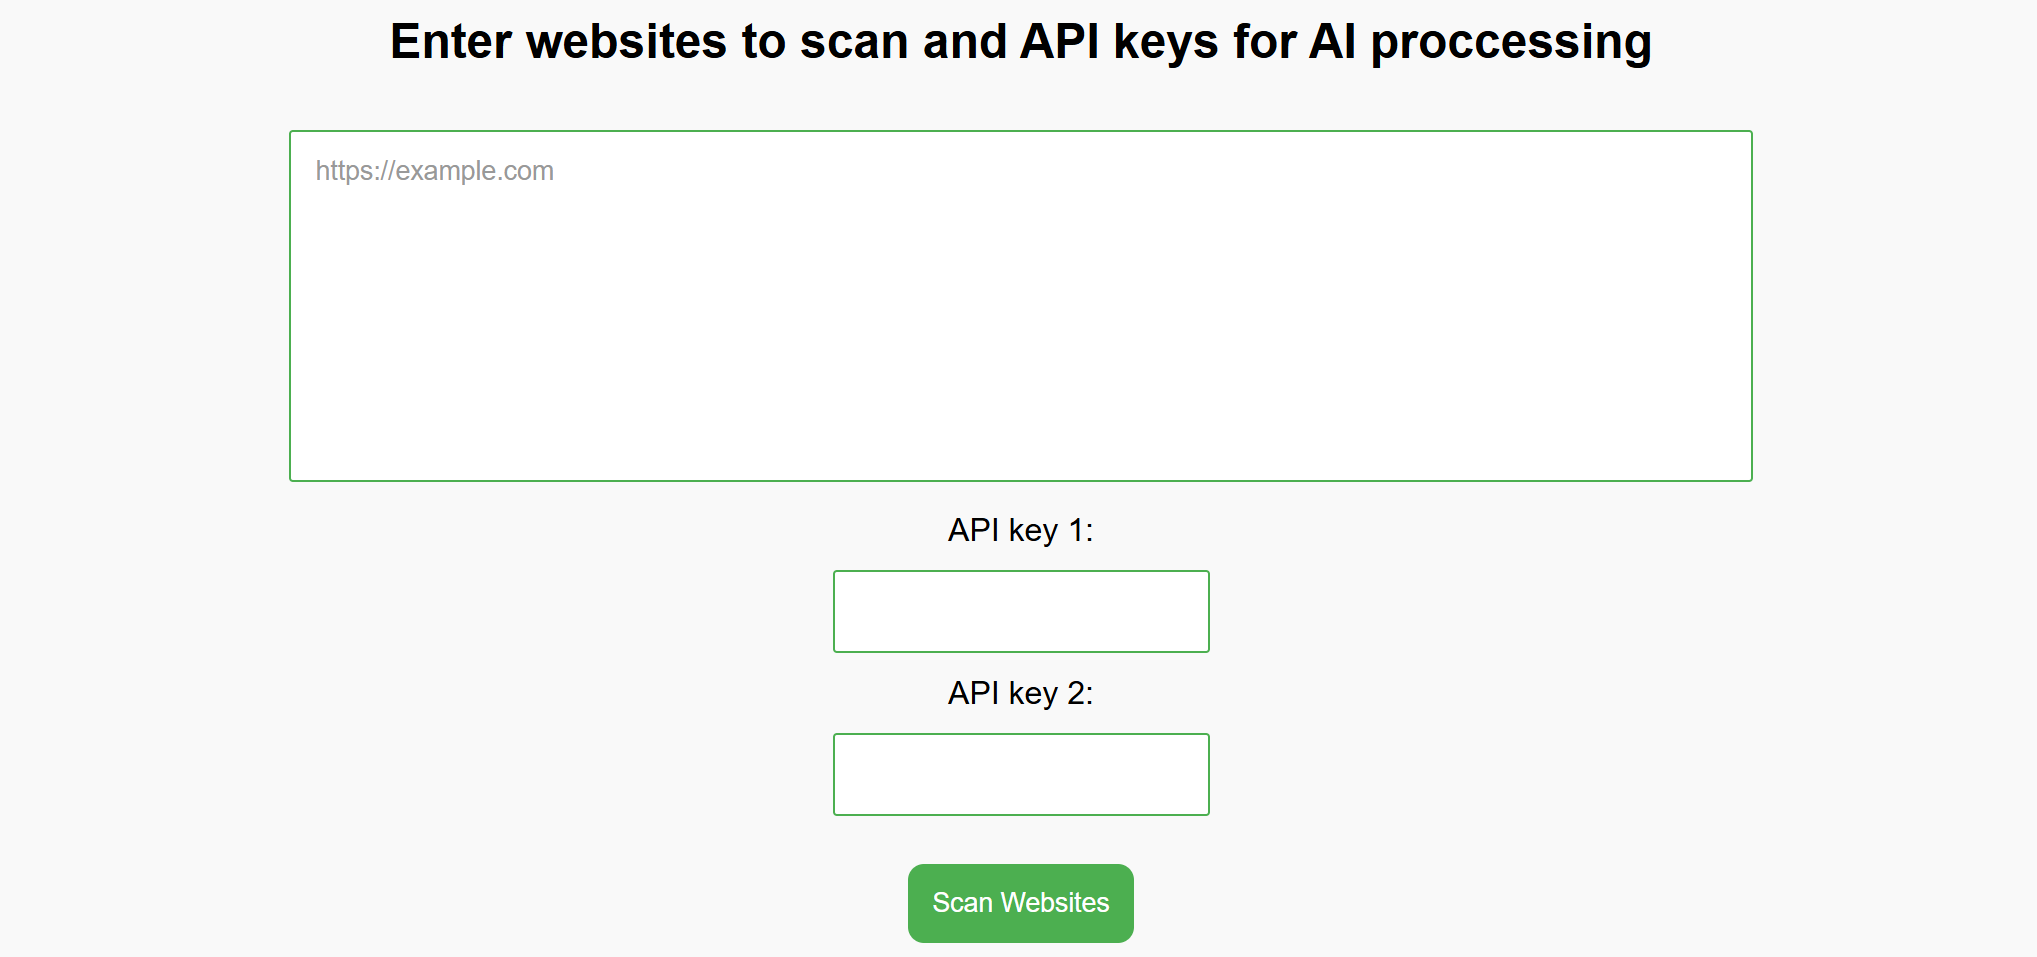
\includegraphics[width=\linewidth]{images/index.png}
        \caption{Úvodní rozhraní}
        \label{fig:index.png}
    \end{figure}

    \clearpage
    \item[Výsledkové rozhraní:] Tato část aplikace slouží k analýze obsahu jednotlivých webových stránek. U každé URL adresy jsou zobrazeny odkazy na ToS, nalezené licence a extrahovaný text. Jak je patrné z návrhu na Obrázku \ref{fig:scans.png}, uživatel zde může vybrat API službu a požádat o sumarizaci obsahu pomocí tlačítka „Generate Summary“.  
    \begin{figure}[H]
        \centering
        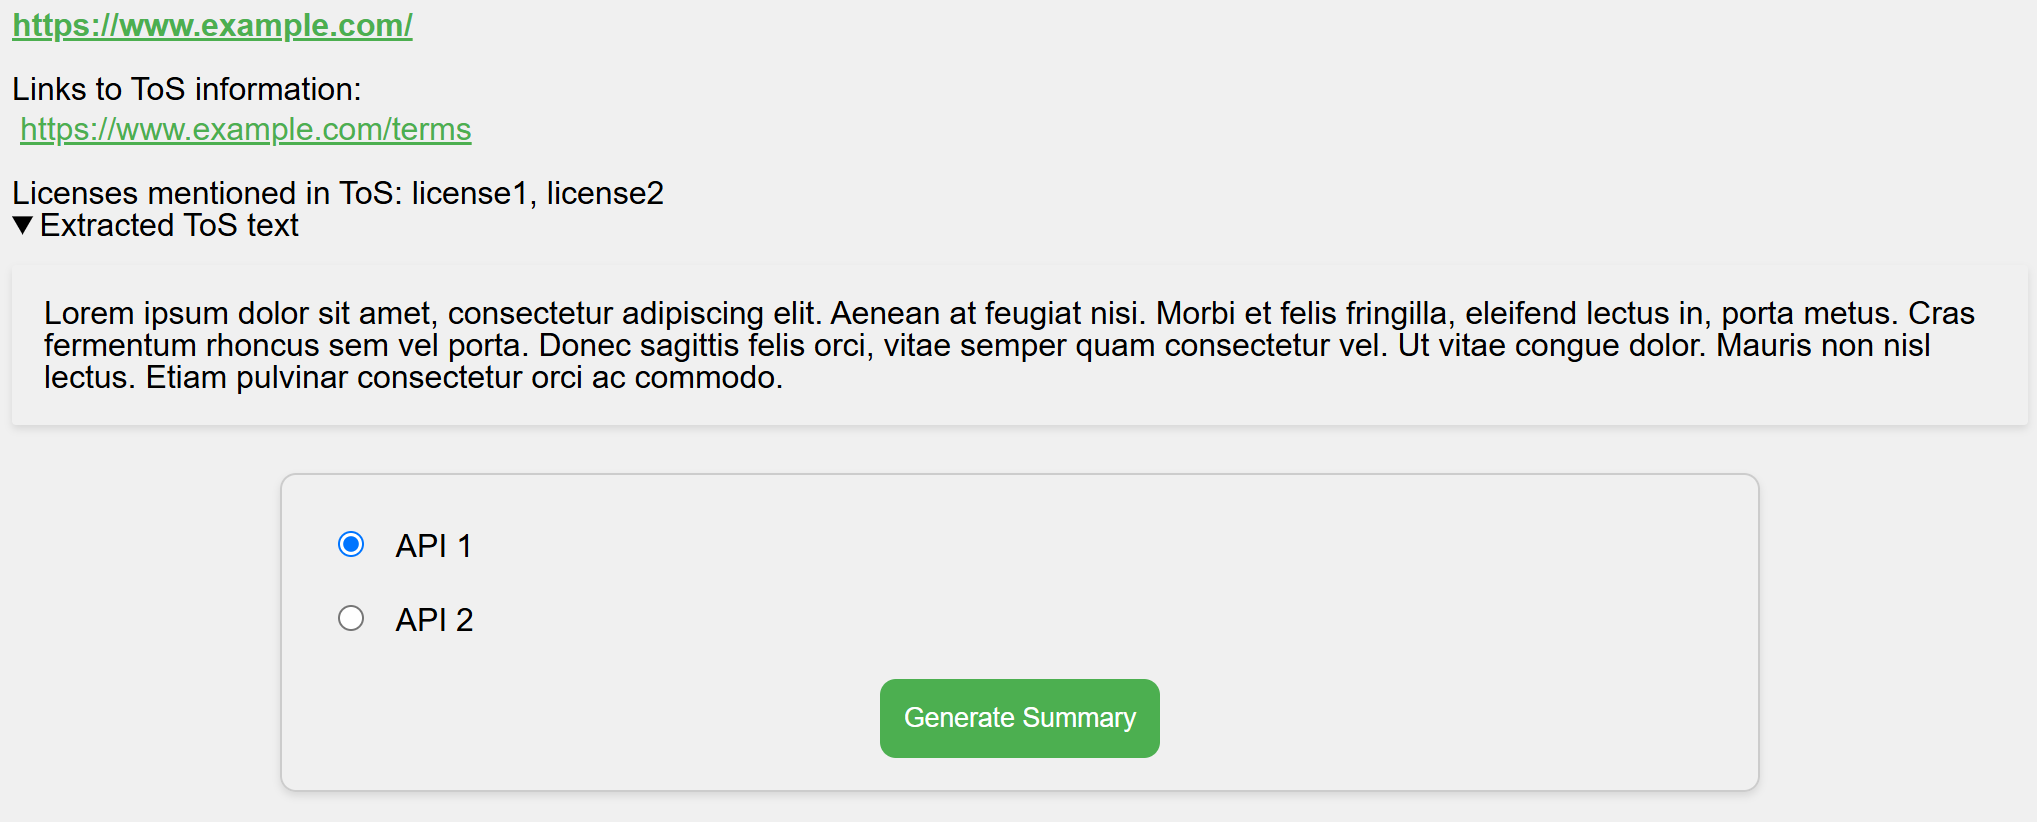
\includegraphics[width=\linewidth]{images/scans.png}
        \caption{Výsledkové rozhraní}
        \label{fig:scans.png}
    \end{figure}

    \item[Rozhraní souhrnu:] Po vygenerování sumarizace je uživateli zobrazen shrnutý text a formulář pro kladení doplňujících otázek. Na Obrázku \ref{fig:summary.png} je zachycen návrh této sekce, kde lze zadat otázku, zvolit API službu pro zpracování a následně získat odpověď přímo na stejné stránce.  
    \begin{figure}[!htbp]
        \centering
        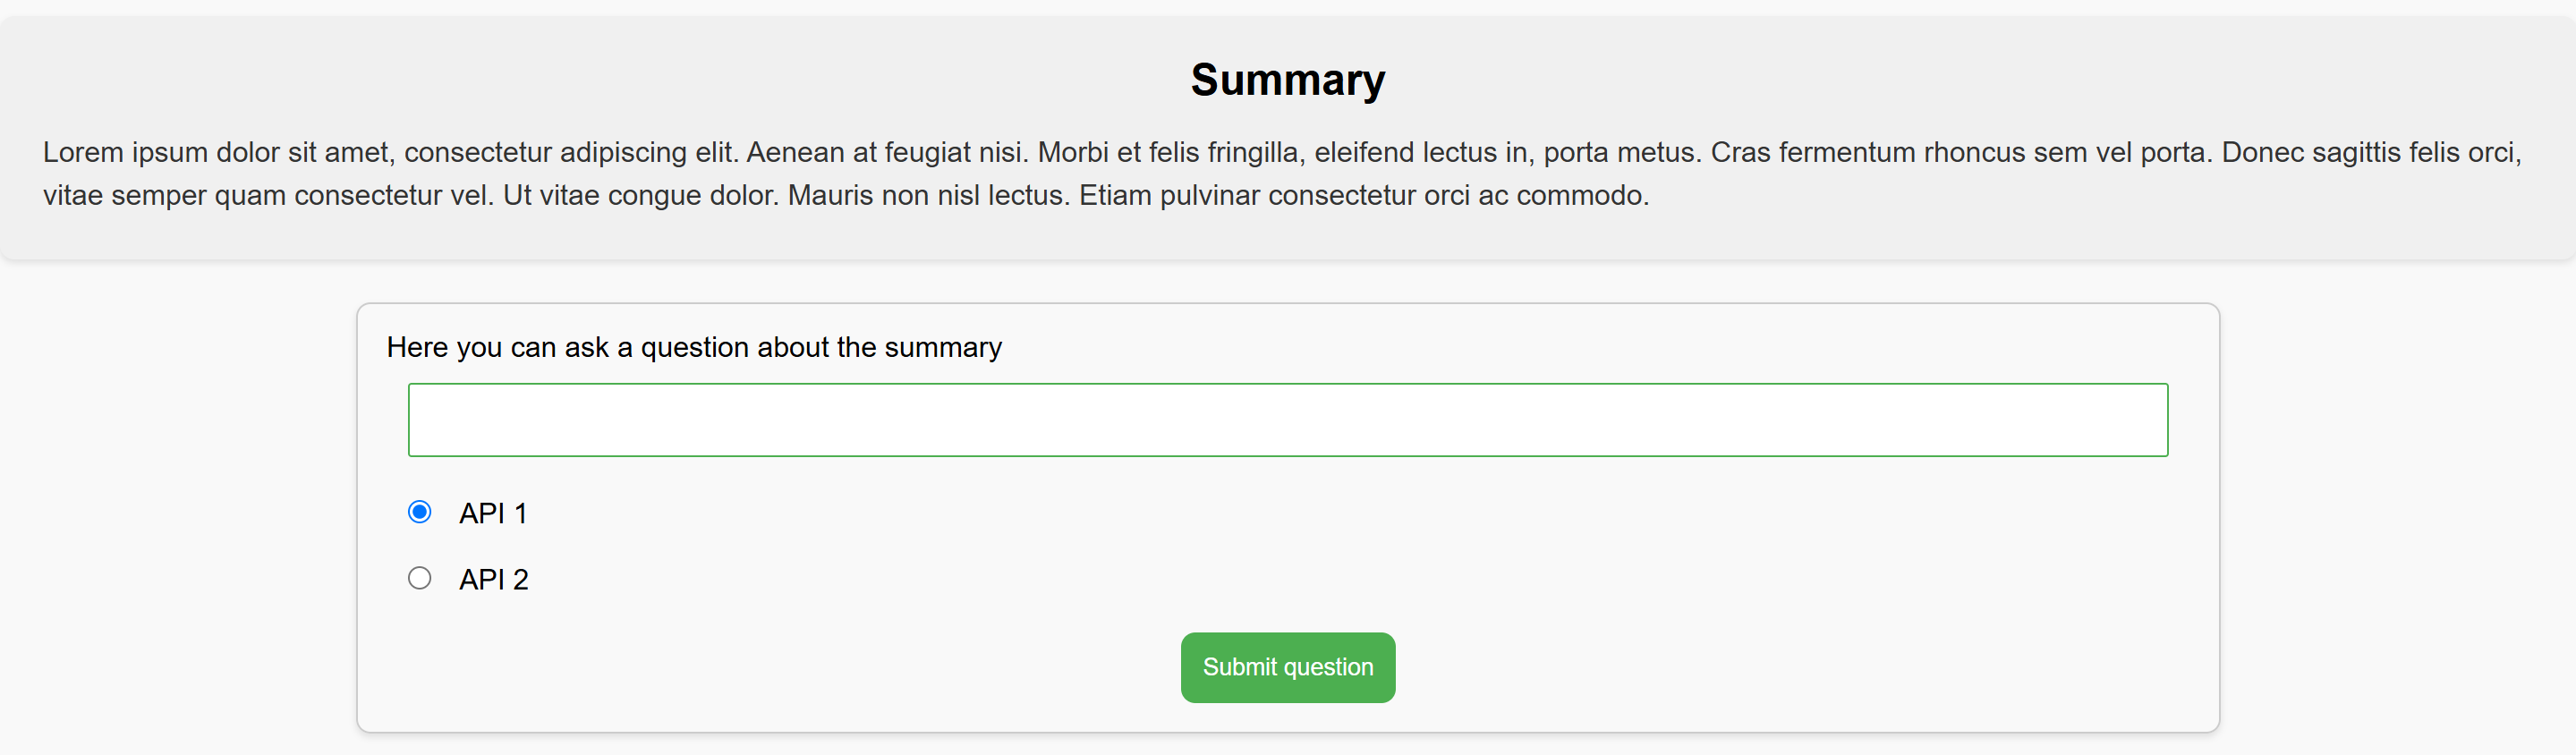
\includegraphics[width=\linewidth]{images/summary.png}
        \caption{Rozhraní souhrnu}
        \label{fig:summary.png}
    \end{figure}
\end{description}


%---------------------------------------------------------------

%---------------------------------------------------------------
\chapter{Implementace}
\begin{chapterabstract}
    Tato kapitola popisuje praktickou realizaci navrhovaného nástroje.
    Zaměřuje se na výběr technologií, strukturu modulů, implementaci klíčových funkcionalit a vývoj prototypu webové aplikace.
    Představeny jsou také detaily formátu výstupů a volby parametrů pro detekci licencí a zpracování ToS.
\end{chapterabstract}

\section{Výběr technologií}
Pro implementaci nástroje se využívá programovací jazyk Python, který tvoří základ nejen navrhované knihovny, ale také prototypu webové aplikace.
Níže je přehled hlavních používaných technologií:

\begin{description}
    \item[Python] Zvolen pro svou univerzálnost a rozsáhlý ekosystém knihoven pro web scraping a zpracování přirozeného jazyka. Navíc je široce používaný v oblasti strojového učení a umělé inteligence, což z něj činí ideální volbu pro práci s jazykovými modely.
    \item[Requests] Knihovna pro odesílání HTTP požadavků a získávání obsahu webových stránek \cite{requestsRequestsHTTP}. V rámci nástroje se používá pro načítání HTML obsahu stránek včetně dokumentu robots.txt a zajištění správného nastavení UA pro web scraping.
    \item[BeautifulSoup] Knihovna pro parsování HTML a extrakci informací z webových stránek \cite{crummyBeautifulSoup}. Umožňuje efektivní prohledávání DOM objektů a identifikaci prvků, jako jsou odkazy na ToS nebo CC licence.
    \item[Huggingface_hub] Knihovna pro přístup k jazykovým modelům z platformy Hugging Face \cite{huggingfaceClientLibrary}. Využívá se pro svůj široký výběr open source modelů a snadnou integraci v rámci Python prostředí.
    \item[Google-genai] Knihovna pro interakci s API rozhraním generativní umělé inteligence společnosti Google \cite{googleapisGoogleDocumentation}. Oproti Hugging Face tak reprezentuje proprietární alternativu pro zpracování textu a generování odpovědí.
    \item[Flask] Lehký webový framework pro vývoj backendu \cite{palletsprojectsWelcomeFlask}. Byl zvolen pro svou jednoduchost a schopnost rychle vytvořit funkční rozhraní potřebné pro prototyp webové aplikace.
    \item[Celery] Nástroj pro správu asynchronních úloh na pozadí \cite{celeryqCeleryDistributed}. Využívá se ke zpracování časově náročných operací, jako je sumarizace ToS textů v rámci API dotazů.
    \item[Redis-py] Python klient pro databázi Redis \cite{redisRedispy600}. V implementaci zajišťuje efektivní správu fronty úloh pro Celery a ukládání dočasných výsledků.
\end{description}

\section{Moduly}
Implementace je rozdělena do čtyř hlavních modulů: Správa požadavků, Extrakce dat, Identifikace licence a Zpracování ToS.
První tři moduly jsou integrovány do centrální třídy \textit{LicenseDetector}, která je vstupním bodem celé knihovny.
Tato třída inicializuje příslušné komponenty a řídí jejich spolupráci při zpracování webového obsahu prostřednictvím metody \textit{scan_websites}, jež přijímá seznam URL adres a vrací výsledky analýzy.

Modul Zpracování ToS je navržen jako samostatná komponenta využívající jazykové modely pro analýzu podmínek použití.
Není přímo propojen s \textit{LicenseDetector}, což umožňuje jeho nezávislé použití v různých kontextech.

Následující podkapitoly podrobně popisují implementaci jednotlivých modulů, včetně jejich klíčových funkcí a technických detailů.

\subsection{Správa požadavků}
Modul pro správu požadavků zajišťuje komunikaci s webovými servery a zároveň dbá na dodržování etických zásad při přístupu k webovým stránkám.
Je implementován prostřednictvím třídy \textit{RequestManager}, která pro správu HTTP požadavků využívá knihovnu requests.
Při inicializaci třídy \textit{RequestManager} dochází k vytvoření relace, která umožňuje efektivní opakované odesílání požadavků a správu stavových informací napříč jednotlivými dotazy.
Klíčové funkce modulu zahrnují:

\begin{description}
    \item[Ověření přístupu podle \textit{robots.txt}:] Metoda \textit{is_allowed_by_robots} kontroluje, zda je pro danou URL a UA povolen web scraping. Pokud soubor \textit{robots.txt} není dostupný, modul předpokládá, že přístup je povolen.
    \item[Načítání souboru \textit{robots.txt}:] Metoda \textit{fetch_robots} získává obsah souboru \textit{robots.txt} z dané URL adresy s využitím knihovny Protego \cite{pypiClientChallenge}.
    \item[Načítání webových stránek:] Metoda \textit{fetch_page} načítá obsah webové strán\-ky ze zadané URL adresy. Využívá HTTP GET požadavek a zpracovává případné chyby, jako je neplatná odpověď serveru nebo překročení časového limitu spojení.
    \item[Správa User-Agent:] Metody \textit{set_user_agent} a \textit{get_user_agent} umožňují správu hlavičky User-Agent, což je užitečné při testování vlastního UA.
\end{description}

Tento modul tak tvoří základ pro další komponenty nástroje, které závisí na získání a ověření webového obsahu.

\subsection{Extrakce dat}
Modul pro extrakci dat je zodpovědný za zpracování HTML obsahu webových stránek a získávání relevantních informací, jako jsou odkazy na licence a ToS.
Je implementován třídou \textit{DataExtractor}, která využívá knihovnu BeautifulSoup pro parsování HTML struktury.
Třída je navržena tak, aby fungovala ve spolupráci s modulem pro správu požadavků, který je předán při inicializaci.
Klíčové funkce modulu jsou:

\begin{description}
    \item[Parsování HTML obsahu:] Metoda \textit{parse\_html} převádí surový HTML obsah na objekt \textit{BeautifulSoup}, který umožňuje prohledávání a manipulaci s DOM strukturou stránky.
    \item[Extrakce odkazů z patičky:] Metoda \textit{extract\_footer\_links} prohledává elementy \textit{<footer>} na stránce a identifikuje licenční a ToS odkazy. Odkazy jsou identifikovány na základě klíčových slov a regulárních výrazů.
    \item[Extrakce relevantního textu:] Metoda \textit{extract\_relevant\_text} prochází textový obsah stránek obsažený v elementech \textit{<p>}, \textit{<li>} a \textit{<span>}, které běžně nesou rozvinutý či kontextový text na stránce, na rozdíl od nadpisových elementů. Rozděluje text na věty a vybírá ty, které obsahují klíčová slova. Výsledný text je následně spojen do jednoho řetězce pro další zpracování.
\end{description}

Zmíněná klíčová slova a regulární výrazy jsou definovány v souboru parametrů \textit{parameters.py}, který je popsán v podkapitole \ref{chap:parameters}.
Výběr těchto vzorů probíhal v průběhu vývoje a testování nástroje na různých webových stránkách.
Hlavním cílem bylo vybalancovat přesnost a citlivost detekce, aby bylo možné efektivně identifikovat relevantní odkazy a texty.


\subsection{Identifikace licence}
Modul pro identifikaci licence je zodpovědný za detekci a klasifikaci licencí obsažených v extrahovaném textu nebo odkazech.
Je implementován třídou \textit{LicenseIdentifier}, která vrací identifikované licence ve standardizovaném formátu.
Mezi klíčové funkce modulu patří:

\begin{description}
    \item[Detekce licencí Creative Commons:] Metoda \textit{determine_cc_license} analyzuje zadanou URL adresu a text pro identifikaci CC licencí. Nejprve kontroluje přítomnost licence CC0. Pokud není CC0 nalezena, hledá specifické CC licence v URL na základě kombinací verzí a typů licencí (např. \uv{licenses/by/4.0} pro CC-BY-4.0). Pokud URL neobsahuje licenci, používá regulární výrazy k extrakci licence z textu a mapuje textové názvy na standardní formát (např. \uv{Attribution} na \uv{BY}). Nakonec vrací identifikovanou licenci jako řetězec (např. \uv{CC-BY-4.0}) nebo \uv{Unknown}, pokud licence není nalezena.
    \item[Extrakce obecných licencí:] Metoda \textit{extract_licenses} prohledává zadaný text a hledá shody s předdefinovanými vzory licencí. Každý vzor odpovídá konkrétnímu typu licence (např. \uv{MIT}, \uv{Apache}). Výsledkem je seznam unikátních názvů licencí nalezených v textu.
\end{description}

Oproti původnímu návrhu modulu je implementace rozšířena o detekci jiných typů licencí, než jsou licence Creative Commons.
Motivace pro toto rozšíření vzešla během testování nástroje na různých webových stránkách, kde v rámci textu ToS byly zmíněny i jiné typy licencí.
Díky tomu je nástroj schopen uživateli poskytnout souhrn zmíněných licencí ještě před zpracováním ToS jazykovými modely.

Stejně jako u modulu pro extrakci dat, i zde jsou klíčová slova a regulární výrazy definovány v souboru parametrů.
Tento přístup umožňuje jednoduše pravidla aktualizovat a přizpůsobit bez nutnosti měnit samotný kód modulu.

\subsection{Zpracování ToS}
Modul pro zpracování podmínek použití je dle návrhu implementován jako samostatný modul, který je rozdělen do několika částí.
Hlavní funkcionalitou modulu je zpracování textového obsahu ToS získaného z předchozích modulů a jeho transformace do stručného shrnutí nebo odpovědí na specifické otázky pomocí jazykových modelů.
Klíčové komponenty modulu zahrnují:

\begin{description}
    \item[Správa modelů:] \textit{ModelManager} je factory třída, která slouží jako rozhraní pro výběr a inicializaci jazykových modelů. Umožňuje dynamicky získat instanci modelu na základě jeho názvu. Tato flexibilní konstrukce zajišťuje, že systém lze jednoduše rozšířit o případné další modely.
    \item[Abstraktní třída modelů:] \textit{BaseModel} je abstraktní třída, která definuje společné rozhraní pro všechny jazykové modely. Obsahuje metodu pro přípravu dotazů (promptů), která formátuje vstupní data do podoby vhodné pro model, a metodu pro validaci vstupních dat. Validace zajišťuje, že vstupní data obsahují povinné položky, jako je obsah ToS nebo název webu, čímž se předchází chybám při zpracování.
    \item[Implementace modelu \textit{Mistral}:] Třída \textit{Mistral} integruje model \textit{Mixtral-8x7B-Instruct-v0.1} prostřednictvím knihovny huggingface_hub. Obsahuje metody \textit{summarize} a \textit{answer\_question}, které generují shrnutí a odpovědi na základě zadaného promptu. Třída zároveň zajišťuje ošetření chyb, jako je neplatný API klíč nebo nedostupnost modelu. Výstupem je text, který může být dále zpracován nebo uložen.
    \item[Implementace modelu \textit{Gemini}:] Třída \textit{Gemini} využívá model \textit{gemini-2.5-pro-exp-03-25} prostřednictvím knihovny \textit{google.generativeai}. Stejně jako třída \textit{Mistral} implementuje metody \textit{summarize} a \textit{answer\_question}, které komunikují s modelem přes API a zpracovávají chyby, jako je neplatný API klíč.
\end{description}

Při implementaci tohoto modulu bylo experimentováno s různými jazykovými modely, a to jak open source, tak proprietárními.
Ze skupiny proprietárních modelů byl vybrán \textit{gemini-2.5-pro-exp-03-25} pro svou přístupnost prostřednictvím bezplatného API a svým bezkonkurenčním výsledkům.
Z open source modelů dostupných na bezplatné verzi Hugging Face API (modely do 10GB) byl vybrán \textit{Mixtral-8x7B-Instruct-v0.1}.
Výběr tohoto modelu nebyl tak jednoznačný a probíhal v průběhu detailnějšího testování, popsaného v příslušné podkapitole \ref{chap:models}.

Co se týče zvolených promptů pro generování shrnutí a odpovědí na otázky, byly navrženy s důrazem na přesnost a stručnost.
Pro sumarizaci je prompt strukturován tak, aby model obdržel název webu a kompletní text ToS s instrukcí vytvořit shrnutí.
Pro odpovědi na otázky prompt obsahuje souhrn ToS a konkrétní otázku v rámci kontextu shrnutí.
To zajišťuje, že model reaguje na situace, kdy uživatel klade dotazy mimo tematický rámec shrnutí.

\begin{lstlisting}[caption={Metoda \textit{prepare\_prompt} třídy BaseModel},label={lst:prompt}]
def _prepare_prompt(self, data, question=None):
    if question:
        return (
            f"Summary of the Terms of Service text:\n{data['summary']}\n\n"
            f"Answer the following question about the ToS summary:\n{question}"
        )
    return f"Summarize the following Terms of Service text from {data['website']}:\n{data['content']}"
\end{lstlisting}


\section{Formát výsledků}
\label{chap:results_format}
Výstupní data první části nástroje jsou generována již dříve zmíněnou třídou \textit{LicenseDetector}, která shromažďuje a strukturovaně vrací informace o licenčních údajích získaných z analyzovaných webových stránek.
Hlavní metodou pro generování výsledků je \textit{scan\_websites}, která zpracovává seznam URL adres a vrací seznam slovníků, kde každý slovník představuje výsledky pro jednu webovou stránku.
Formát výsledků \ref{lst:results} je navržen tak, aby byl konzistentní a snadno zpracovatelný pro další použití:

\begin{lstlisting}[caption={JSON formát výsledků},label={lst:results}]
[
    {
    "website": "string",
    "invalidUrl": "boolean",
    "blockedByRobotsTxt": "boolean",
    "licenseLink": "string | null",
    "licenseType": "string | null",
    "relevantLinks": [],
    "licenseMentions": [],
    "content": "string | null"
    },
    ...
]
\end{lstlisting}

\begin{description}
    \item[website:] URL analyzované stránky.
    \item[invalidUrl:] Logická hodnota označující, zda byla vstupní URL neplatná.
    \item[blockedByRobotsTxt:] Logická hodnota signalizující, zda byl přístup zablokován pravidly \textit{robots.txt}.
    \item[licenseLink:] URL odkazu na CC licenci.
    \item[licenseType:] Typ CC licence.
    \item[relevantLinks:] Seznam relevantních odkazů (ToS a podobné dokumenty) získaných z patičky stránky.
    \item[licenseMentions:] Seznam názvů licencí nalezených v textovém obsahu relevantních odkazů.
    \item[content:] Extrahovaný textový obsah z relevantních odkazů, který může být dále zpracován jazykovými modely.
\end{description}

Výstupy druhé části nástroje jsou generovány dvěma hlavními metodami třídy \textit{BaseModel}, které jsou implementovány v jednotlivých třídách jazykových modelů.
Metoda \textit{summarize} vrací slovník, který rozšiřuje vstupní data o klíč \textit{summary} se stručným shrnutím textu ToS.
Aby mohla tato metoda fungovat správně, musí vstupní data obsahovat klíče \textit{website} (název webu) a \textit{content} (text podmínek použití získaný v první části nástroje).
Naproti tomu metoda \textit{answer_question} generuje textovou odpověď na konkrétní dotaz, který se týká již vytvořeného shrnutí.
Pro její správné fungování je vyžadováno, aby vstup obsahoval klíč \textit{summary} spolu s položkou \textit{question}, která formuluje otázku k danému shrnutí.

\clearpage
\section{Definice parametrů}
\label{chap:parameters}
Soubor \textit{parameters.py} slouží jako jednotné místo pro definici klíčových slov a regulárních výrazů využívaných při detekci i extrakci licencí, odkazů a textů ToS.
Následující texty popisují jednotlivé části tohoto souboru:

\begin{lstlisting}[caption={Klíčová slova pro odkazy a textový obsah ToS},label={lst:keywords}]
RELEVANT_LINKS_KEYWORDS = ["terms", "legal", "license", "licensing", "use", "policy", "copyright"]
RELEVANT_TEXT_KEYWORDS = [
    "intellectual property", "right", "authorised", "commercial use", "non-commercial use",
    "fair use", "license", "copyright", "creative commons", "cc by", "gpl", "apache", "mit", "bsd"]
\end{lstlisting}
Tyto konstanty definují klíčová slova pro modul \textit{DataExtractor}.
První obsahuje slova pro identifikaci odkazů v patičkách webových stránek vedoucích k ToS. 
Druhá zahrnuje slova pro extrakci textového obsahu souvisejícího s licenčními informacemi.

\begin{lstlisting}[caption={Parametry licencí Creative Commons},label={lst:cc_parameters}]
CC_VERSIONS = ['1.0', '2.0', '2.5', '3.0', '4.0']
CC_TYPES = ['BY', 'BY-SA', 'BY-ND', 'BY-NC', 'BY-NC-SA', 'BY-NC-ND']
CC_TYPE_MAP = {
    'attribution': 'BY', 'by': 'BY', 'noncommercial': 'NC', 'non-commercial': 'NC', 'nc': 'NC',
    'sharealike': 'SA', 'share-alike': 'SA', 'sa': 'SA', 'noderivatives': 'ND', 'no-derivatives': 'ND', 'nd': 'ND'}
\end{lstlisting}
Tyto konstanty definují parametry pro zpracování CC licencí.
První specifikuje podporované verze licencí, druhá uvádí dostupné typy licencí, a třetí mapuje textové popisy (např. „attribution“ na „BY“) pro standardizaci výstupů. 

\begin{lstlisting}[caption={Regulární výraz pro Creative Commons},label={lst:cc_pattern}]
CC_PATTERN = re.compile(
    r'\b(?:CC[\s-]+(?:(?:BY|Attribution|SA|' 
    r'Share[\s-]?Alike|NC|Non[\s-]?Commercial|' 
    r'ND|No[\s-]?Derivatives)[\s-]?)+'
    r'(?:\d\.\d)?|'
    r'Creative[\s-]+Commons[\s-]*(?:'
    r'(?:Attribution|Share[\s-]?Alike|' 
    r'Non[\s-]?Commercial|No[\s-]?Derivatives|'
    r'BY|SA|NC|ND)[\s-]*)*'
    r'(?:\d\.\d)?|CC0)\b',
    re.IGNORECASE)
\end{lstlisting}
Výraz pro detekci CC licencí rozpoznává tři varianty:
\begin{enumerate}
    \item „CC“ následované jedním nebo více atributy (např. „BY“, „SA“) a volitelným číslem verze (např. „4.0“).
    \item „Creative Commons“ s volitelnými atributy a číslem verze.
    \item Samostatné „CC0“.
\end{enumerate}

Tento a následující regulární výrazy slouží k identifikaci licencí prostřednictvím modulu \textit{LicenseIdentifier}.
Základ těchto výrazů vychází ze seznamu licencí \cite{spdxSPDXLicense}.

\begin{lstlisting}[caption={Regulární výraz pro MIT License},label={lst:mit-pattern}]
MIT_PATTERN = re.compile(
    r'\bMIT[-\s]+(?:\w+\s+){0,3}(?:License|Variant)',
    re.IGNORECASE)
\end{lstlisting}
Tento výraz pro detekci MIT licence rozpoznává text začínající „MIT“ následovaný mezerou nebo pomlčkou, případně až třemi dalšími slovy, a končící slovem „License“ nebo „Variant“.

\begin{lstlisting}[caption={Regulární výraz pro Apache License},label={lst:apache-pattern}]
APACHE_PATTERN = re.compile(
    r'\bApache[-\s]+(?:License[-\s]*'
    r'(?:v?\d+(?:\.\d+)?)?|v?\d+(?:\.\d+)?)\b',
    re.IGNORECASE)
\end{lstlisting}
Tento výraz detekující Apache licenci rozpoznává text začínající „Apache“ následovaný mezerou nebo pomlčkou, po kterém může následovat buď „License“ s volitelným číslem verze (např. „2.0“), nebo přímo číslo verze (např. „v2.0“).

\begin{lstlisting}[caption={Regulární výraz pro GNU GPL},label={lst:gpl-pattern}]
GPL_PATTERN = re.compile(
    r'\b(?:GNU[\s-]+(?:A|L)?GPL|'
    r'(?:A|L)?GPL[\s-]*(?:v?\d+(?:\.\d+)?)|'
    r'General\s+Public\s+License)\b',
    re.IGNORECASE)
\end{lstlisting}
Tento výraz pro detekci GNU GPL rozpoznává tři varianty:
\begin{enumerate}
    \item „GNU“ následované „GPL“ s volitelným prefixem „A“ nebo „L“.
    \item „GPL“ s volitelným prefixem „A“ nebo „L“ a číslem verze (např. „v3“ nebo „2.0“).
    \item Plný název „General Public License“.
\end{enumerate}

\clearpage
\begin{lstlisting}[caption={Regulární výraz pro BSD License},label={lst:bsd-pattern}]
BSD_PATTERN = re.compile(
    r'\bBSD[\s-]+(?:\d+[\s-]Clause|License)\b',
    re.IGNORECASE)
\end{lstlisting}
Tento výraz detekující BSD licenci rozpoznává text začínající „BSD“ následovaný mezerou nebo pomlčkou, po kterém následuje buď číslo a „Clause“ (např. „2-Clause“) nebo slovo „License“.

\section{Prototyp webové aplikace}
Prototyp je implementován jako jednoduché, avšak funkční rozhraní, které umožňuje uživatelům zadávat URL adresy, zobrazovat výsledky analýzy licenčních informací, generovat shrnutí a odpovídat na otázky týkající se ToS.
Implementace je dle návrhu rozdělena na backend, který zpracovává požadavky a komunikuje s moduly nástroje, a frontend, který zajišťuje interaktivní uživatelské rozhraní.
\subsection{Backend}
Backend prototypu je implementován pomocí dříve zmiňovaného frameworku Flask.
Hlavní komponenty jsou pak definovány v několika třídách, které společně zajišťují routování, logiku zpracování a komunikaci s databází.
Klíčové části backendu zahrnují:

\begin{description}
    \item[Routování požadavků:] Třída \textit{Router} definuje následující cesty pro zpracování HTTP požadavků:
    \begin{itemize}
        \item / \\
        Zobrazuje domovskou stránku (\textit{index.html}) s formulářem pro zadání URL adres a API klíčů.
    
        \item /scans/<scan_id> \\
        Načítá výsledky analýzy z databáze podle scan_id a zobrazuje je v šabloně \textit{scans.html}.
        Tato cesta je cílem přesměrování z POST požadavku \textit{/scans}, který inicializuje analýzu stránek metodou \textit{scan_websites} třídy \textit{Services}.
    
        \item /scans/<scan_id>/summaries/<summary_id> \\
        Načítá shrnutí ToS z databáze podle \textit{summary_id} a zobrazuje ho v šabloně \textit{summary.html}.
        Tato cesta je cílem přesměrování z POST požadavku \textit{/scans/<scan_id>/summaries}, který generuje shrnutí metodou \textit{summarize_results} třídy \textit{Services} na základě vybraného API (huggingface nebo googleai).
    
        \item /scans/<scan_id>/summaries/<summary_id>/answers/<answer_id> \\
        Načítá shrnutí a odpověď na otázku z databáze podle \textit{summary_id} a \textit{answer_id} a zobrazuje je opět v šabloně \textit{summary.html}.
        Tato cesta je cílem přesměrování z POST požadavku \textit{/scans/<scan_id>/summaries/\allowbreak<summary_id>/answers}, který generuje odpověď metodou \textit{answer_question} třídy \textit{Services}.
    \end{itemize}
    
    \item[Logika zpracování:] 
      Třída \textit{Services} zajišťuje integraci s moduly nástroje a koordinaci operací. 
      Klíčové funkce zahrnují:

      \begin{itemize}
        \item \textit{scan_websites:} Volá metodu \textit{scan\_websites} třídy \textit{LicenseDetector} pro analýzu stránek, 
          ukládá výsledky do databáze prostřednictvím třídy \textit{Database} a vrací \textit{scan\_id}.
        \item \textit{summarize_results:} Parsuje výsledky detekce, volá metodu \textit{summarize} vybraného jazykového modelu 
          ukládá shrnutí do databáze a vrací \textit{summary\_id}.
        \item \textit{answer_question:} Načítá shrnutí z databáze, volá metodu \textit{answer\_question} vybraného modelu, 
          ukládá odpověď do databáze a vrací \textit{answer\_id}.
        \item Validace vstupů: Zajišťuje kontrolu URL adres, API klíčů a formátu dat. V případě neplatných vstupů vyhazuje výjimky, které jsou 
          zpracovány na úrovni routování.
      \end{itemize}
    
    \item[Správa dat:] 
      Třída \textit{Database} zpracovává všechny operace s databází, včetně ukládání a načítání výsledků analýzy, shrnutí a odpovědí.
      Data jsou ukládána pouze dočasně a po určité době jsou automaticky odstraněna.
  \end{description}
  
Ačkoli původní návrh prototypu nepředpokládal použití databáze, velký objem textových dat v podobě extrahovaného obsahu stránek a shrnutí ToS motivoval k zavedení databázového systému pro efektivní správu a uchovávání těchto dat. 
Z tohoto důvodu byla zvolena jednoduchá databáze Redis, která je rychlá a efektivní pro ukládání dočasných dat.
Redis je rovněž využíván v rámci asynchronního zpracování požadavků prostřednictvím Celery v rozhraní API, jak je popsáno v podkapitole \ref{chap:api} níže, což umožňuje konzistentní správu dat napříč celou aplikací.

Pro zlepšení uživatelského zážitku byla při routování implementována technika Post/Redirect/Get, která zabraňuje opakovanému odesílání formulářů při obnovení stránky a zajišťuje soulad s moderními webovými standardy.

Třída \textit{Services}, přestože je zjednodušena díky oddělení databázové logiky do třídy \textit{Database}, stále koordinuje více operací, jako je validace vstupů, parsování dat a komunikace s modely.
Pro budoucí rozšíření by bylo vhodné zvážit její rozdělení do dílčích služeb na samostatné třídy, aby byla zajištěna větší modularita a snadnější údržba.

\subsection{API}
\label{chap:api}

\begin{description}
    \item[Routování požadavků:] Třída \textit{APIRouter} definuje endpointy \ref{tab:api_endpoints} pro úlohy skenování webových stránek, generování shrnutí ToS a zodpovídání otázek. Požadavky jsou přijímány ve formátu JSON a odpovědi vraceny s odpovídajícími HTTP status kódy.
    \item[Asynchronní zpracování:] Úlohy jsou zpracovávány asynchronně prostřednictvím systému Celery. Třída \textit{APIServices} následně validuje vstupní hodnoty a tyto úlohy zpracovává.
  \end{description}
  

Celery je systém určený pro plánování a řízení výpočetně náročných úloh, který umožňuje jejich oddělení od hlavního aplikačního toku.
V této implementaci hraje klíčovou roli Redis databáze, která slouží jako broker i jako úložiště výsledků.
Celý tento mechanismus je znázorněn na následujícím diagramu \ref{fig:celery_diagram}.
\begin{figure}[H]
    \centering
    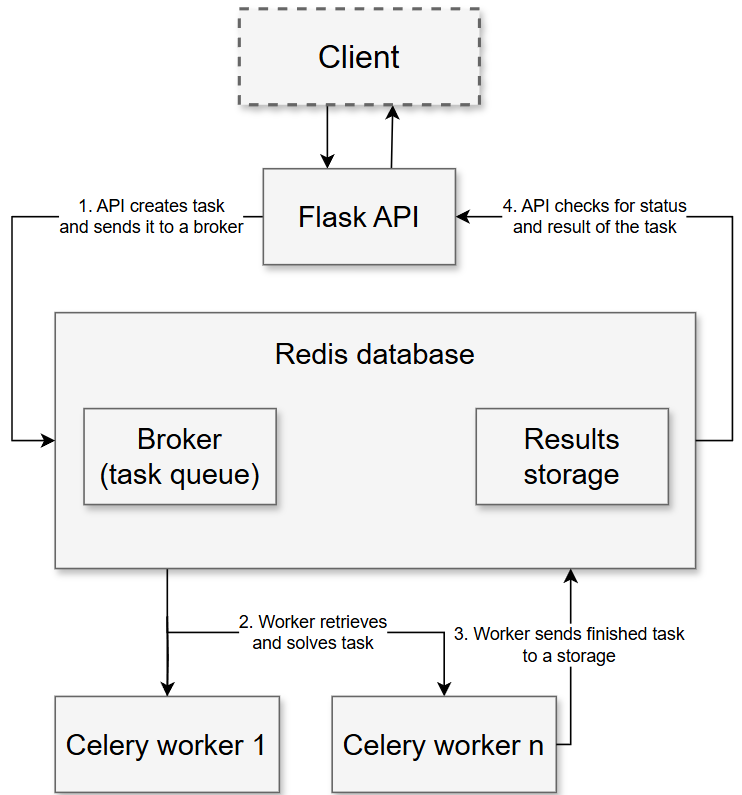
\includegraphics[width=\linewidth]{images/celery.png}
    \caption{Celery diagram}
    \label{fig:celery_diagram}
\end{figure}

Broker (zprostředkovatel) je komponenta, která zajišťuje komunikaci mezi API a Celery workery.
Když API přijme požadavek na zpracování úlohy, nepředává ji workerovi přímo, ale odesílá ji do Redis brokera, který funguje jako fronta zpráv.
Workeři pak z této fronty odebírají úlohy, zpracovávají je a výsledky opět ukládají do Redis úložiště, odkud si je může aplikace nebo klient později vyžádat.

Tímto způsobem je možné úlohy zpracovávat asynchronně a paralelně, což znamená, že uživatel není nucen čekat na jejich dokončení.
Po odeslání úlohy klient obdrží HTTP kód 202 (Accepted) spolu s identifikátorem úlohy, pomocí kterého může sledovat její stav a v případě dokončení, si výsledek úlohy vyzvednout.
Samopopisné stavy úloh, se kterými se uživatel může setkat, jsou: PENDING, SUCCESS, FAILURE, RETRY a REVOKED.

\subsection{Frontend}

Frontend prototypu webové aplikace je implementován pomocí šablonovacího systému Jinja \cite{palletsprojectsJinjax2014}, který zajišťuje dynamické generování obsahu na základě dat předaných z backendu.
Bez využití samostatného frontendového frameworku, je rozhraní navrženo jako jednoduché, ale funkční, a v rámci prototypu dostačující.
Klíčové šablony jsou definovány v souborech \textit{index.html}, \textit{scans.html} a \textit{summary.html}, které tvoří základ uživatelského rozhraní.
Mezi funkcionality frontendu patří:
\begin{description}
    \item[Zadávání vstupních dat:] Šablona \textit{index.html} obsahuje formulář pro zadání seznamu URL adres webových stránek a API klíčů pro jazykové modely. Uživatel vkládá URL adresy do textového pole a API klíče do vstupních polí typu \textit{password}.
    
    \item[Zobrazení výsledků analýzy:] Šablona \textit{scans.html} prezentuje výsledky analýzy licencí pro každou zadanou URL adresu v přehledných kartách. Každá karta zobrazuje informace, jako je adresa webu, stav (např. blokování souborem \textit{robots.txt}, neplatná URL), nalezené odkazy na licence, typ licence, relevantní odkazy na ToS a extrahovaný text podmínek použití. Uživatel může rozbalit podrobnosti o ToS a inicializovat generování shrnutí výběrem preferovaného API a odesláním požadavku.
    
    \item[Zobrazení shrnutí a odpovědí:] Šablona \textit{summary.html} zobrazuje vygenerované shrnutí ToS spolu s použitým API a umožňuje uživateli zadat otázku k shrnutí prostřednictvím formuláře. Vygenerovaná odpověď je následně zobrazena pod samotným dotazem.
  \end{description}
  
Rozhraní je stylováno pomocí CSS souborů, které zajišťují vizuální konzistenci napříč celou aplikací.
Všechny šablony vycházejí ze společné základní struktury definované v souboru \textit{layout.html}, což usnadňuje zachování jednotného vzhledu napříč stránkami.
Interaktivita aplikace je záměrně omezena pouze na formuláře a odkazy, bez použití klientského JavaScriptu.
Veškerá logika je tak zpracovávána na straně serveru, což přispívá k jednoduchosti implementace.
Tento přístup sice omezuje možnosti pokročilejších uživatelských interakcí, nicméně v kontextu prototypu byl vyhodnocen jako plně dostačující.

Vzhled uživatelského rozhraní vychází z předem připravených návrhových obrázků, které sloužily jako podklad pro implementaci jednotlivých šablon.
Následující sekvence obrázků ilustruje typický průchod aplikací:

    \begin{figure}[!htbp]
        \centering
        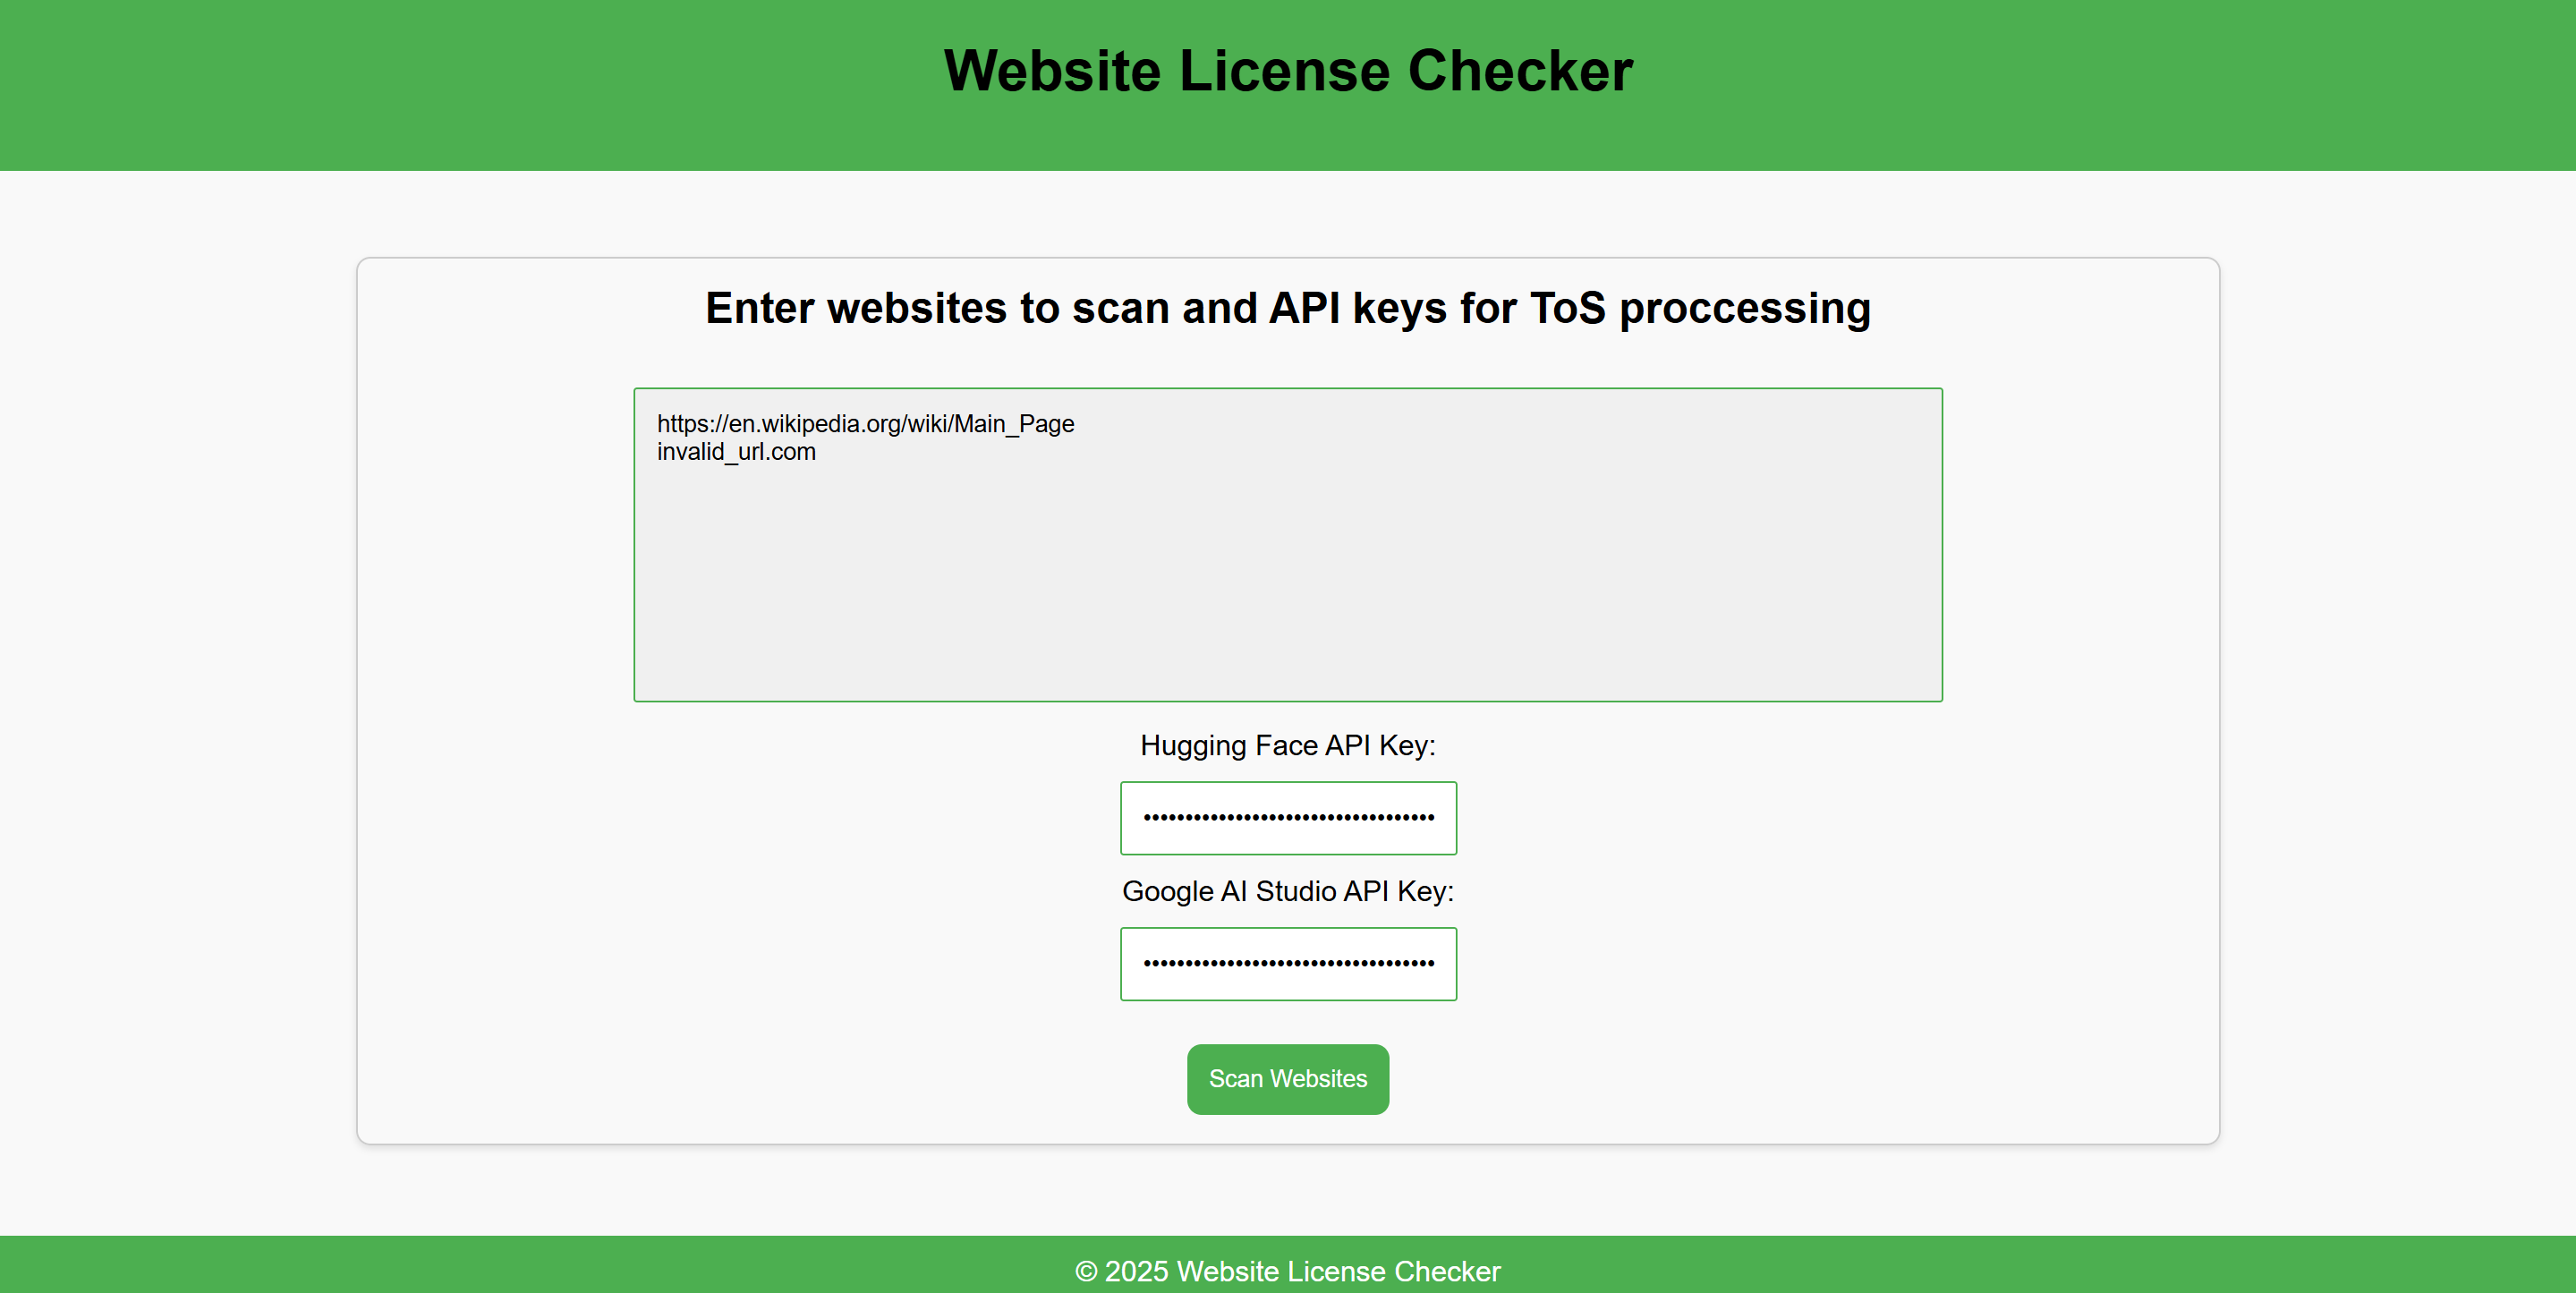
\includegraphics[width=\linewidth]{images/index_imp.png}
        \caption{Odeslání URL adres a API klíčů}
        \label{fig:index_imp.png}
    \end{figure}

    \begin{figure}[!htbp]
        \centering
        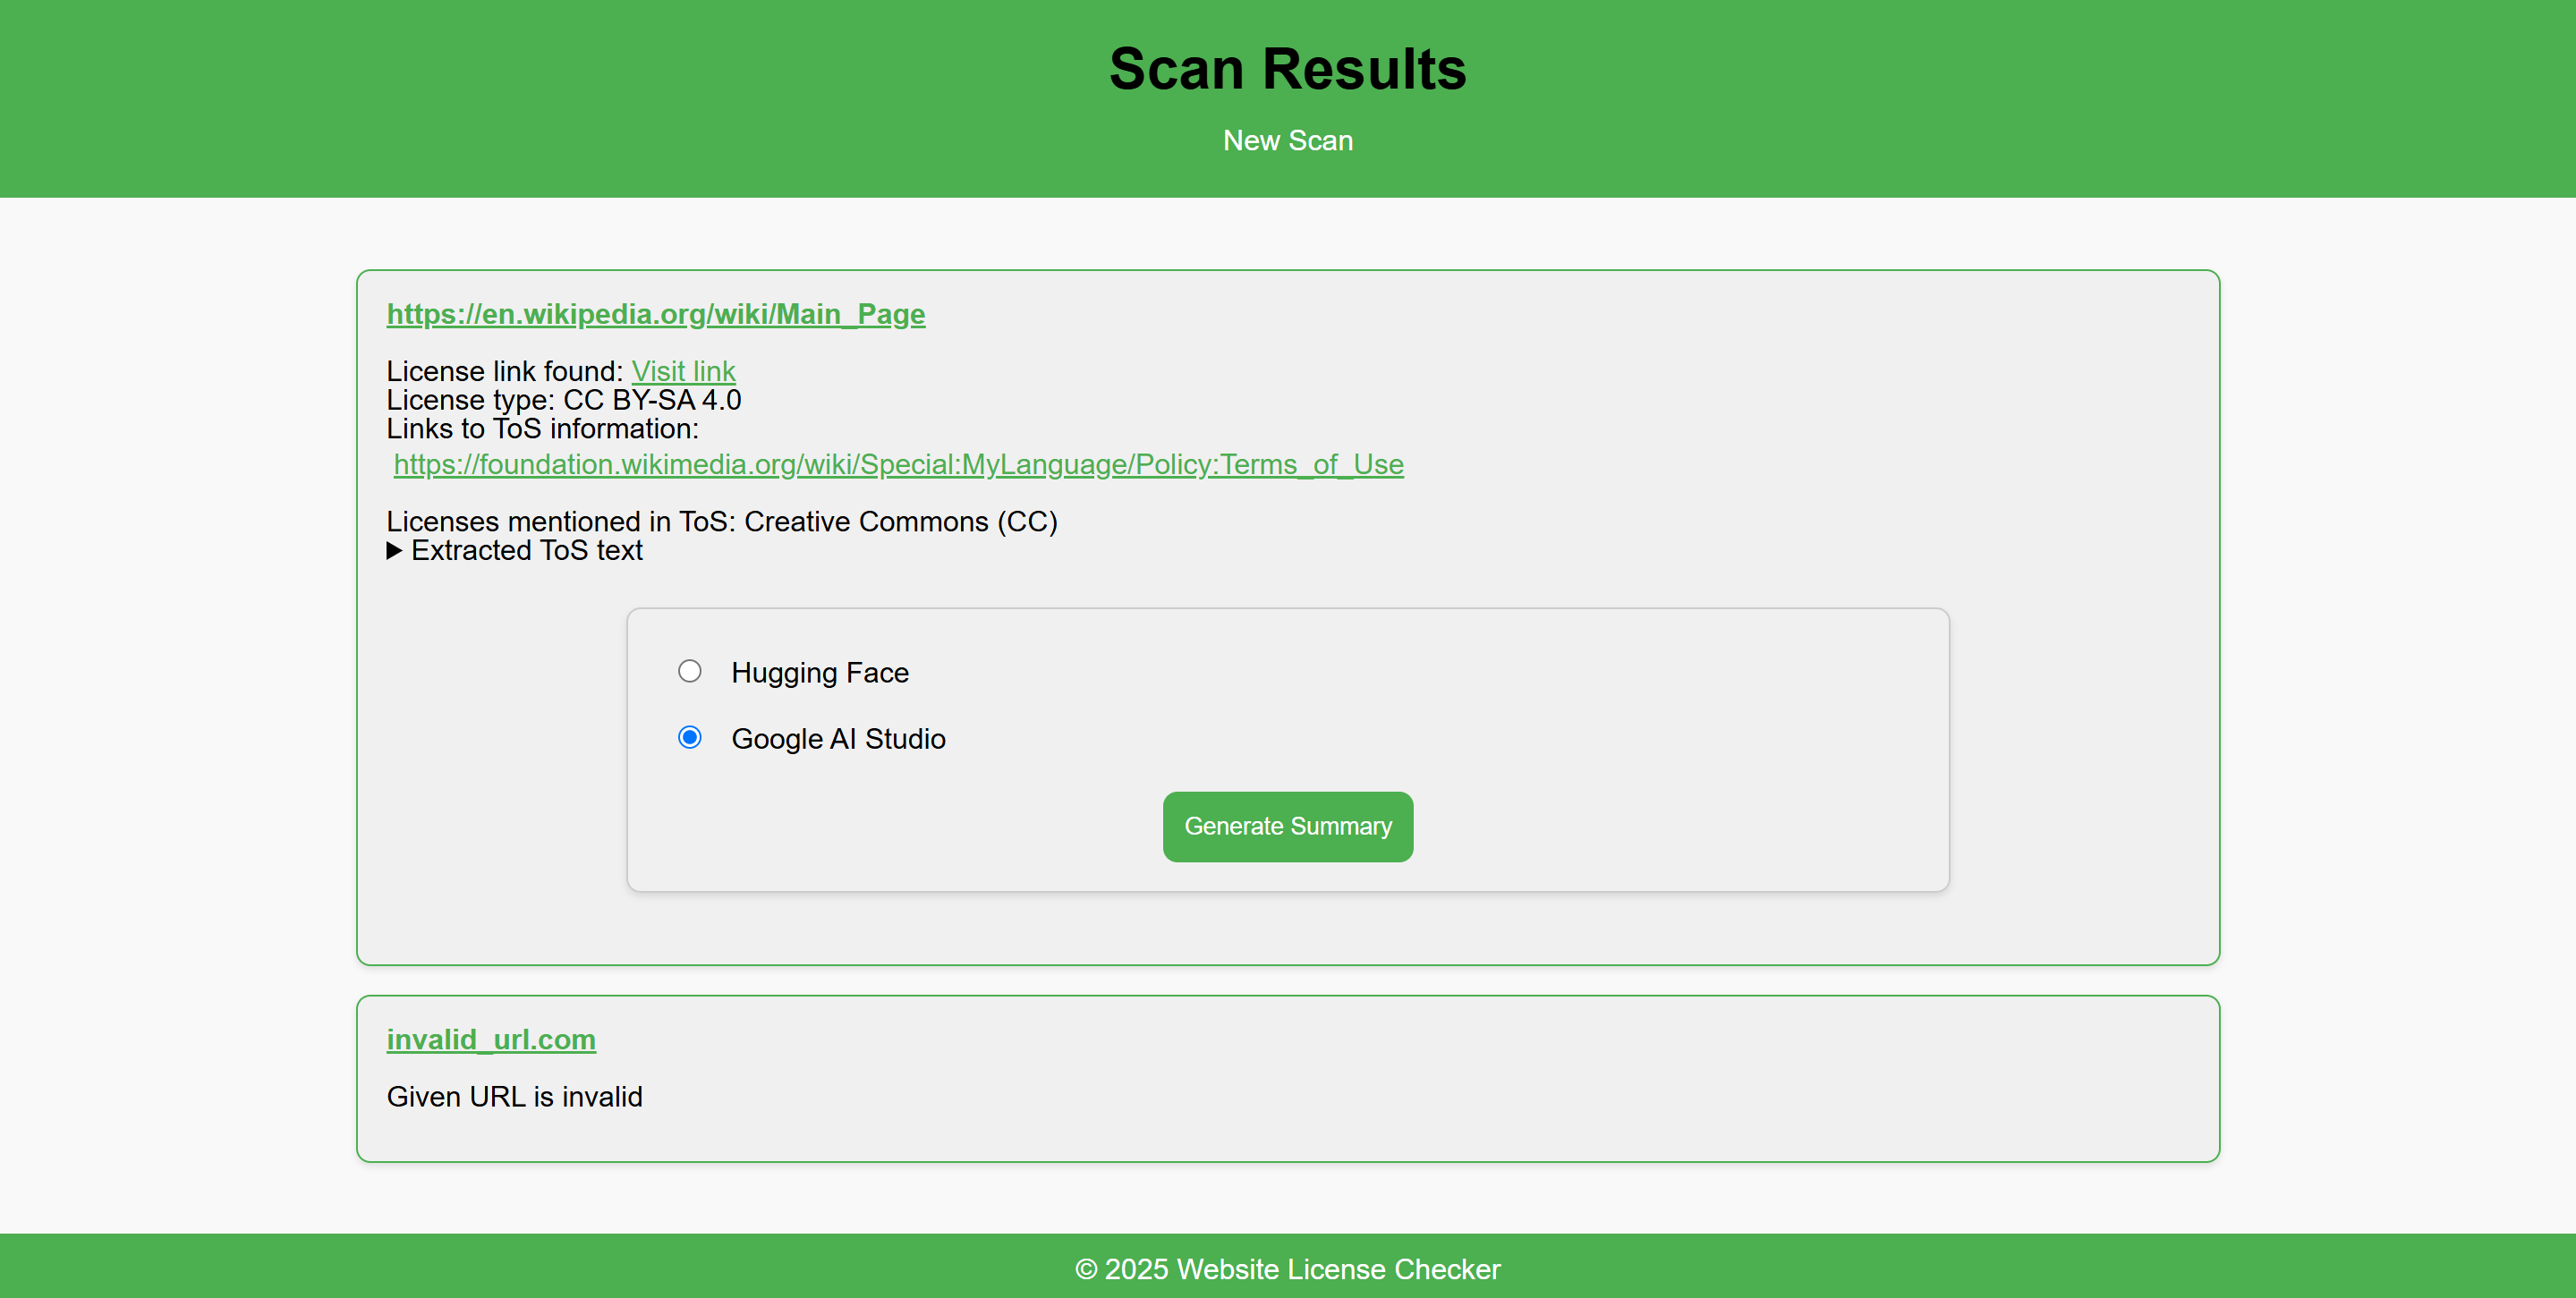
\includegraphics[width=\linewidth]{images/scans_imp.png}
        \caption{Zobrazení výsledků analýzy a možnost summarizovat ToS}
        \label{fig:scans_imp.png}
    \end{figure}

    \begin{figure}[!htbp]
        \centering
        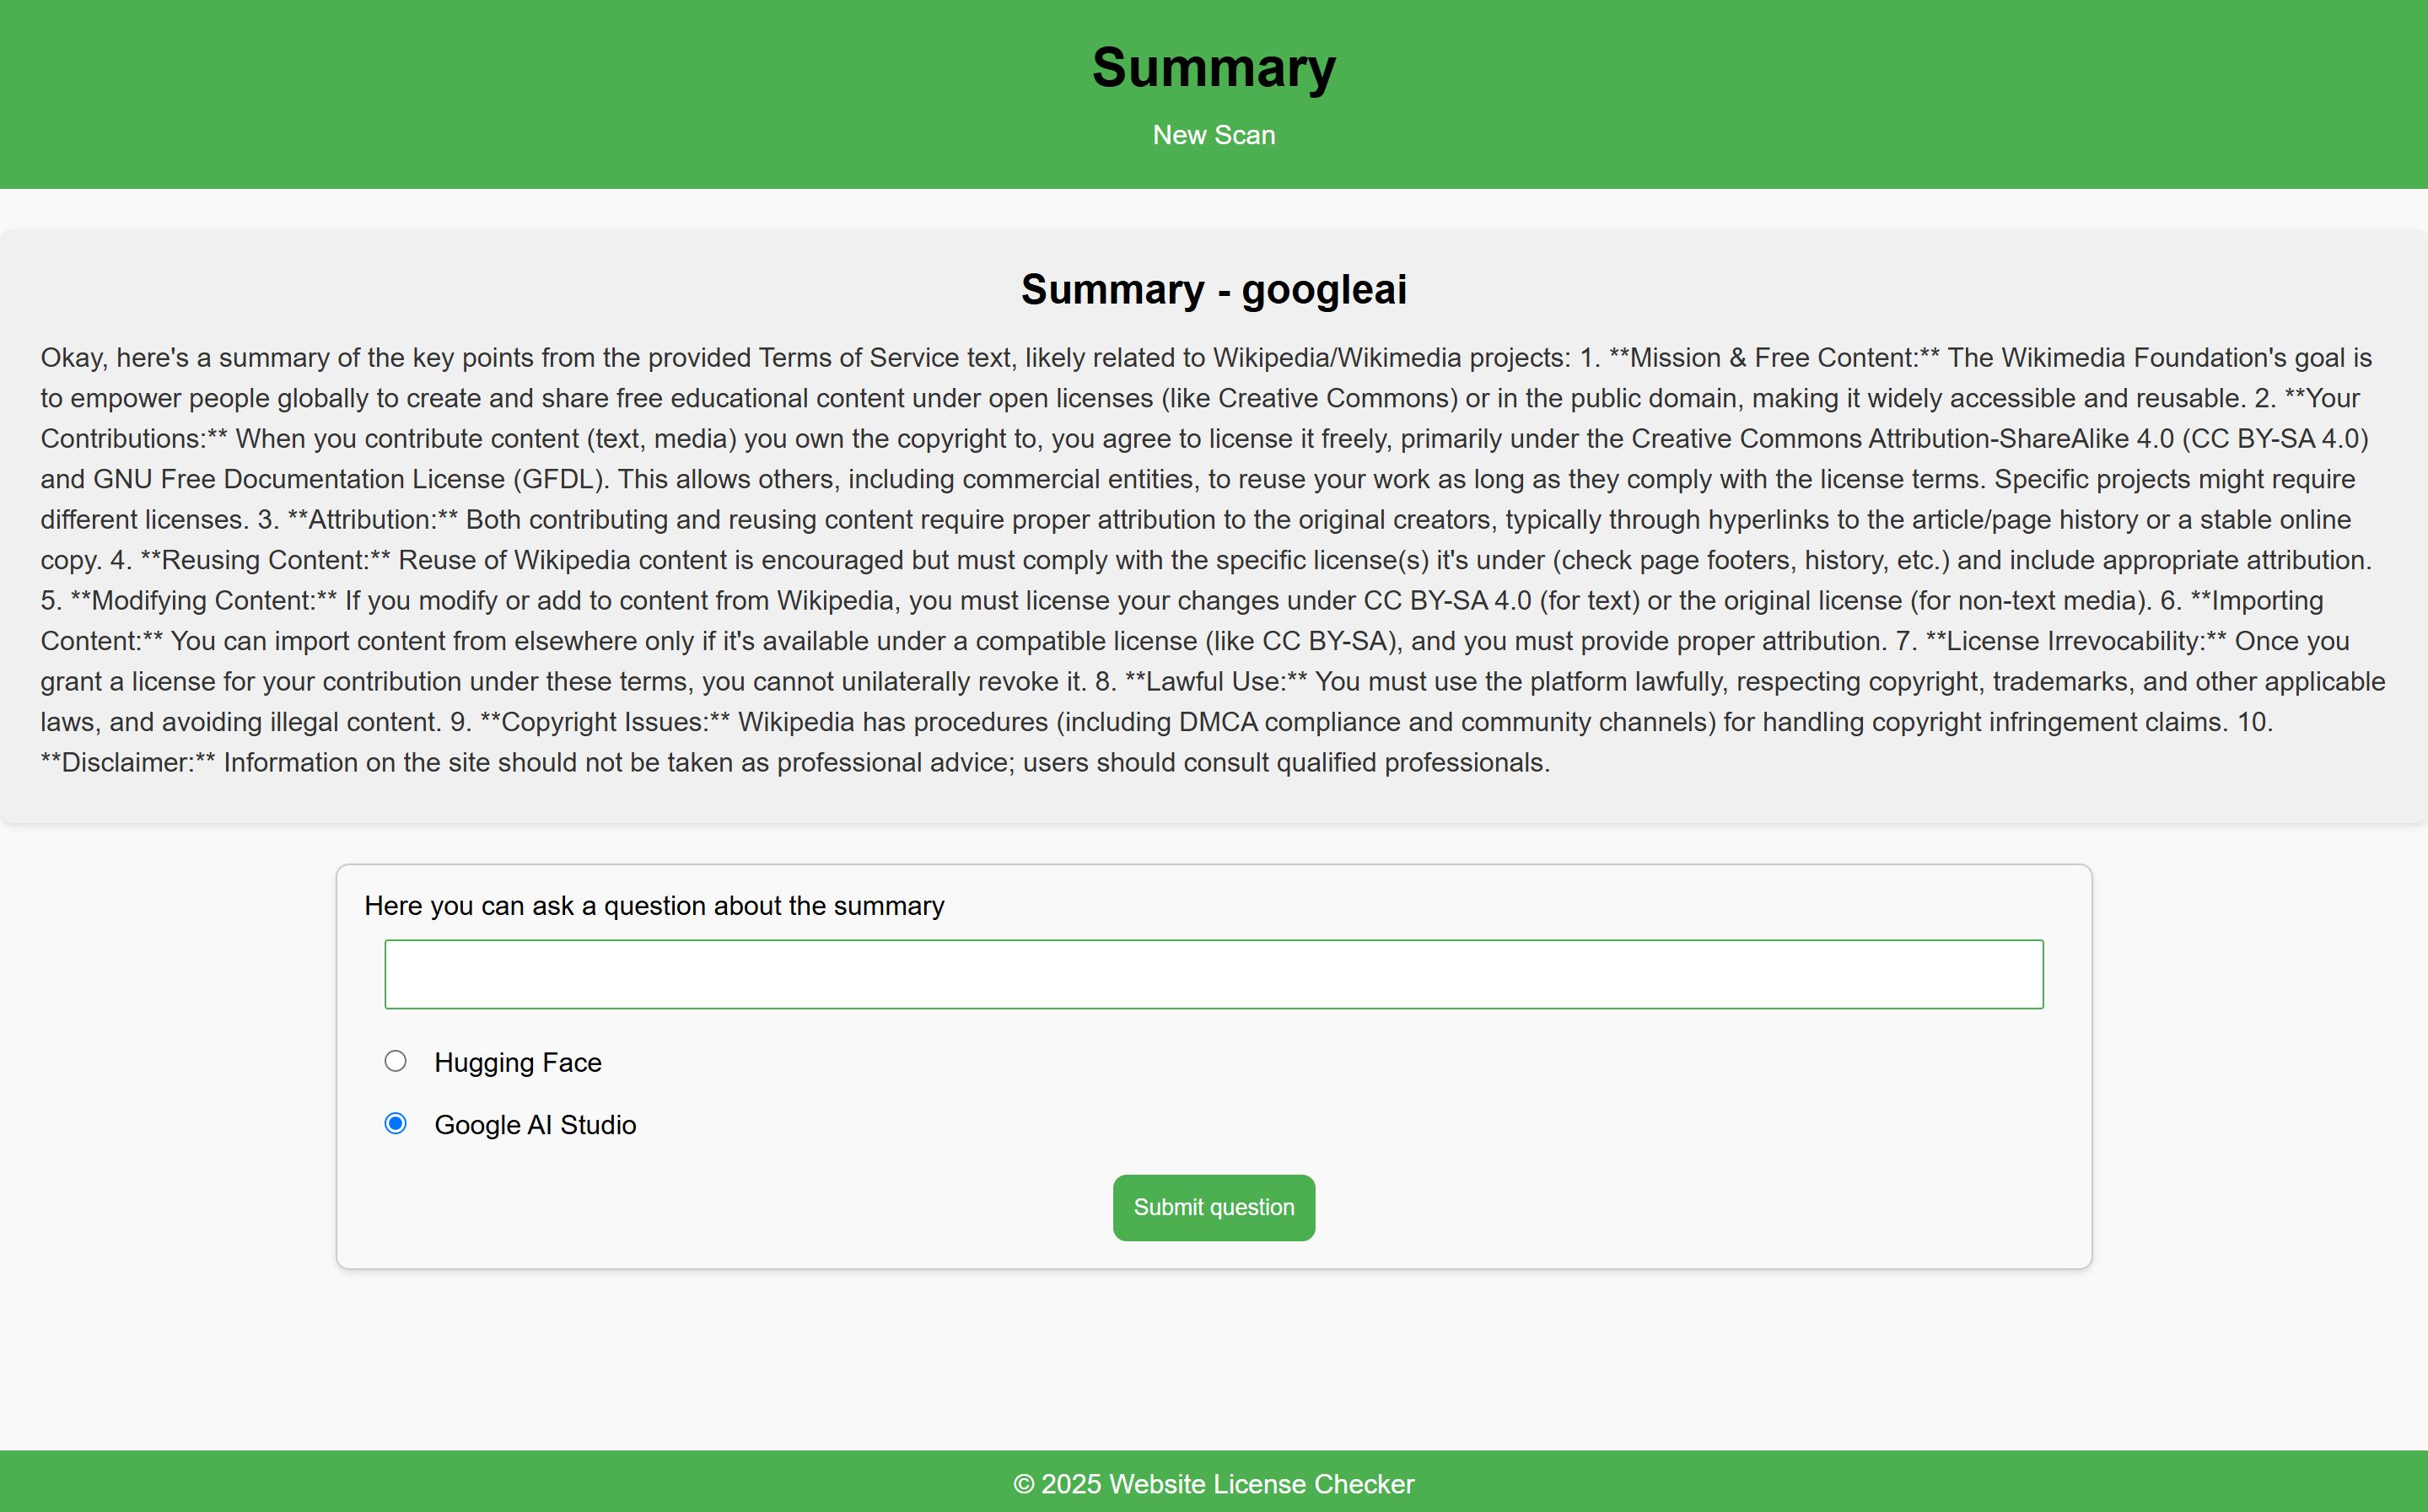
\includegraphics[width=\linewidth]{images/summary_imp.png}
        \caption{Zobrazení shrnutí ToS a možnost položit otázku}
        \label{fig:summary_imp.png}
    \end{figure}

    \begin{figure}[!htbp]
        \centering
        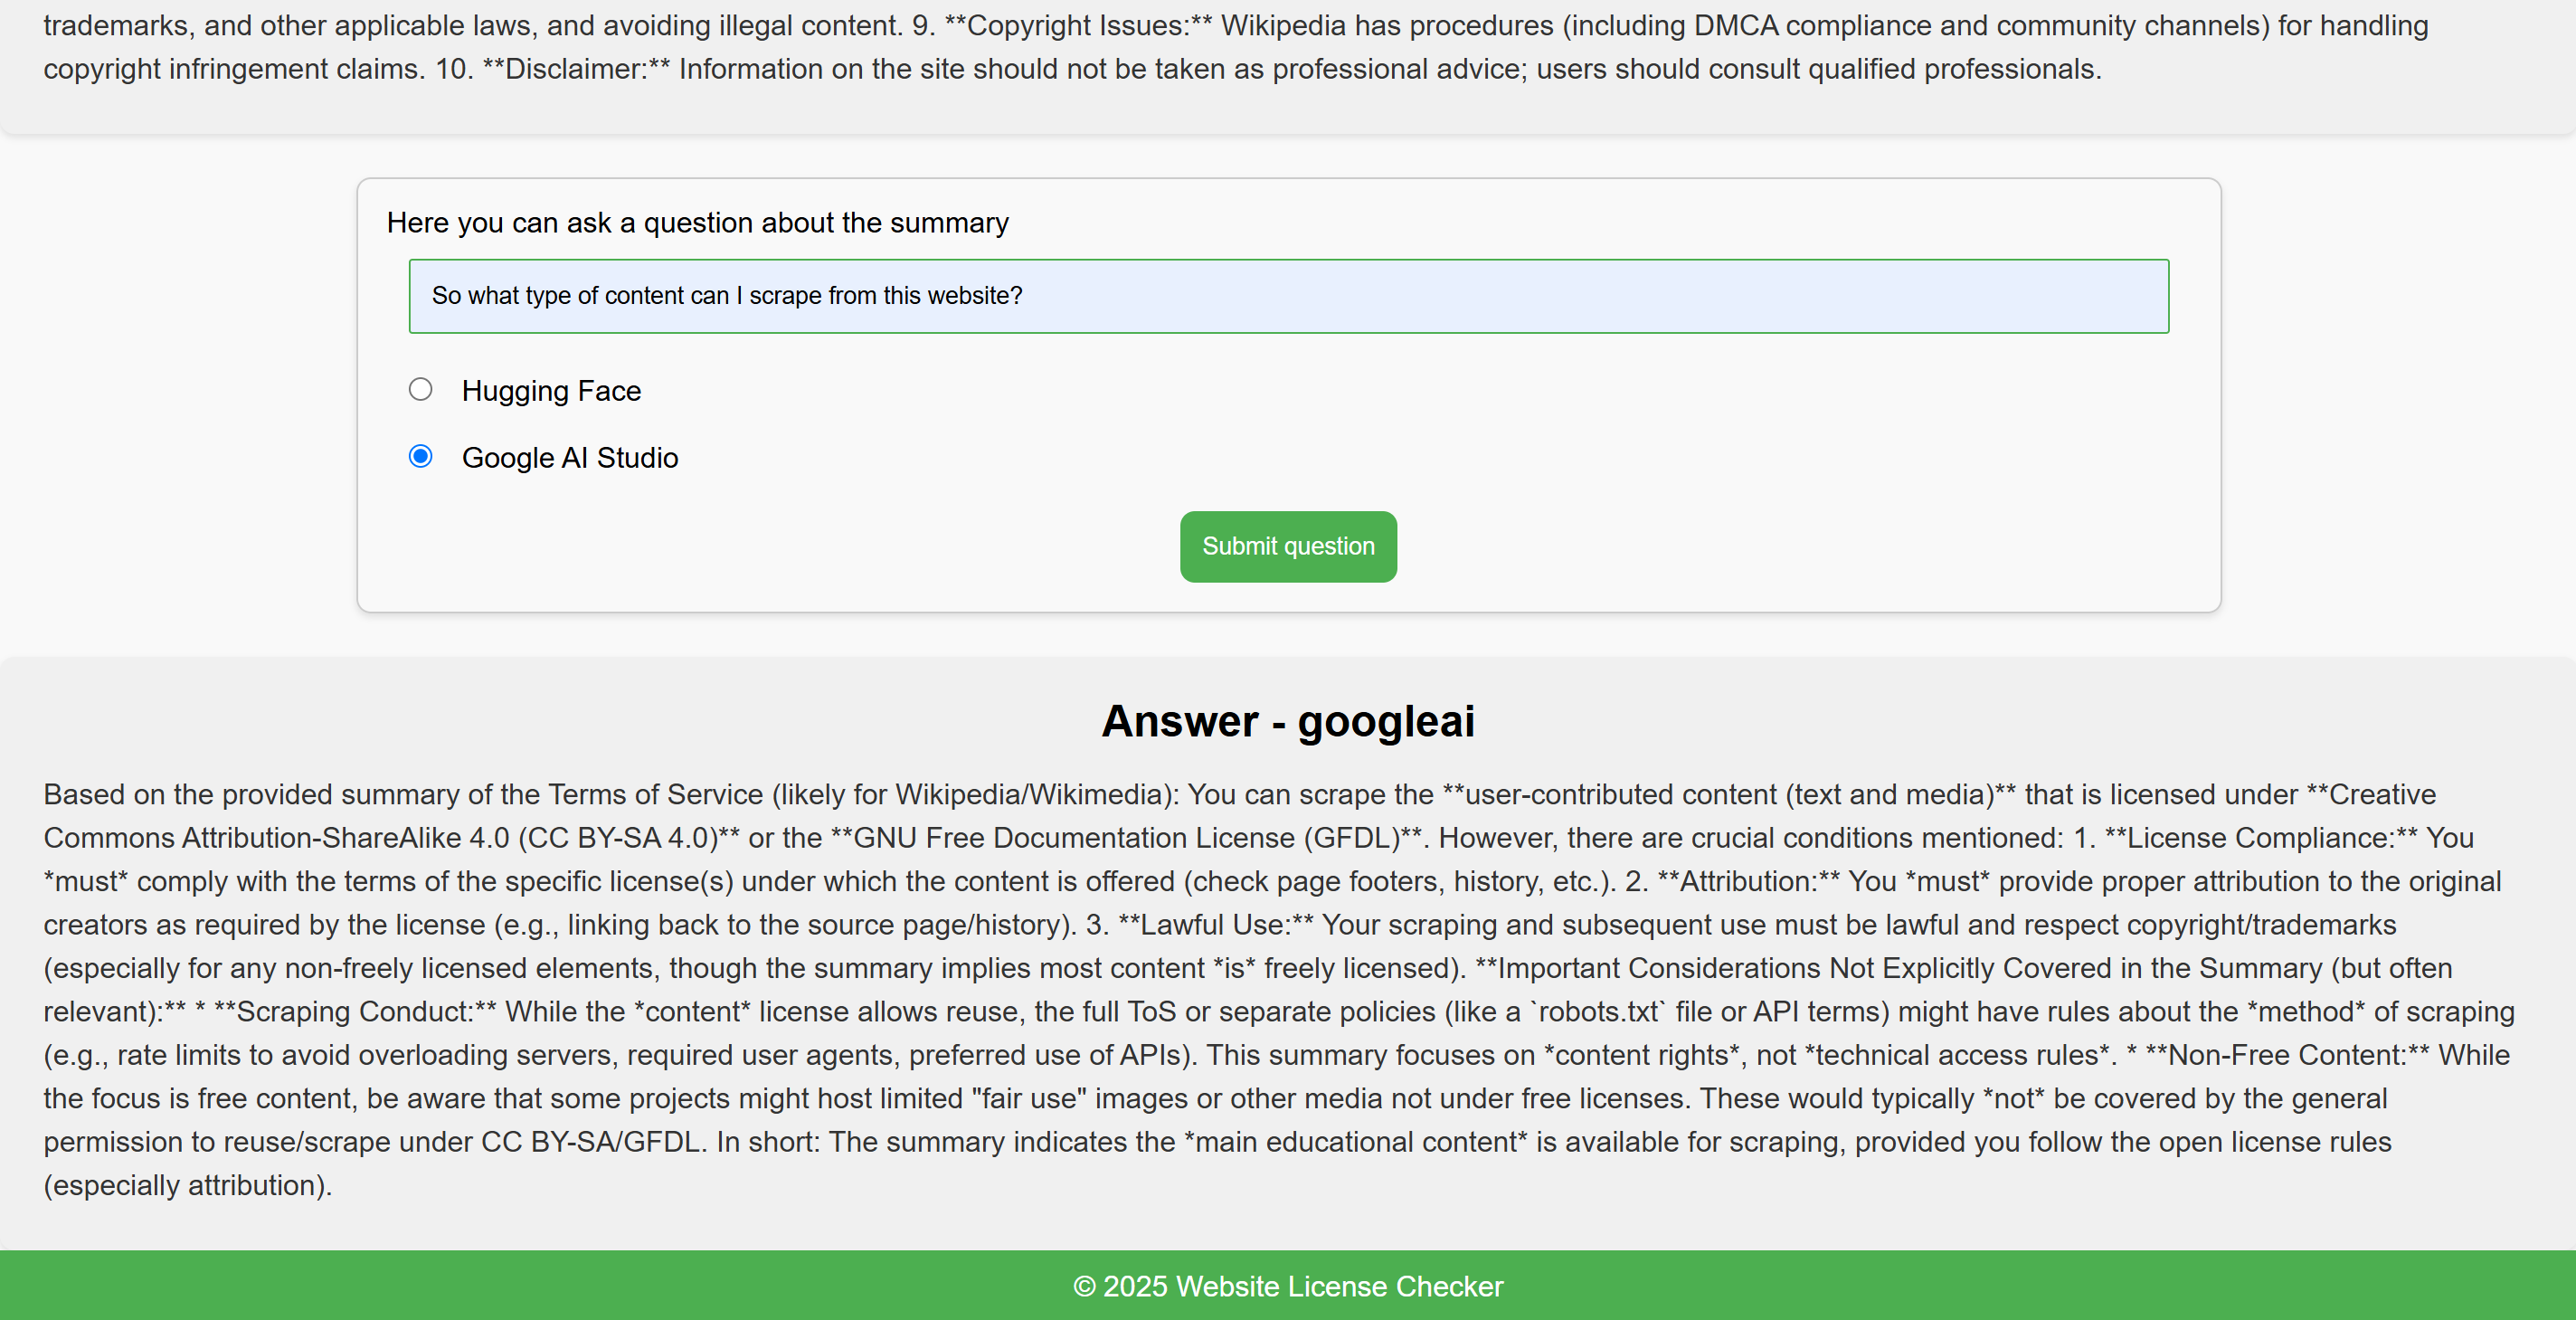
\includegraphics[width=\linewidth]{images/answer_imp.png}
        \caption{Zobrazení odpovědi na otázku a možnost položit další otázku}
        \label{fig:answer_imp.png}
    \end{figure}

  

%---------------------------------------------------------------

%---------------------------------------------------------------
\chapter{Testování}
\begin{chapterabstract}
    Během vývoje byly jednotlivé části knihovny i webové aplikace průběžně manuálně testovány, a to jak prostřednictvím uživatelského rozhraní, tak voláním navrženého API.
    Po dokončení implementace však byla vytvořena i sada automatizovaných testů pomocí nástroje \textit{pytest}.
    Tyto testy ověřují klíčové funkce první části knihovny, jako je kontrola formátu výstupu, zpracování nevalidních vstupů, funkčnost nastavení vlastního UA a respektování pravidel \textit{robots.txt}.
    Avšak hlavní důraz je kladen na testování přesnosti detekce licencí na různých webových stránkách.
    
    Druhá část testování se zaměřuje na hodnocení vyzkoušených open source jazykových modelů.
    K porovnání byly využity standardní metriky jako ROUGE, BERTScore a Faithfulness.
\end{chapterabstract}

\section{Testování detekce}
Během vývoje byly manuálně testovány vybrané webové stránky obsahující licenční informace, jako například \textit{Wikipedia} \cite{wikipediaWikipediaFree}, \textit{Wikiwand} \cite{wikiwandWikiwandWikipedia} a \textit{MDN Web Docs} \cite{mozillaDocs}, aby byla ověřena schopnost knihovny rozpoznat licence v reálných podmínkách.

Pro automatické testy byly během analýzy a studia tématu sbírány další podobné relevantní stránky.
Avšak z důvodu omezeného počtu nalezených stránek bylo přistoupeno k cílenému hledání.
Nejprve byl získán seznam 1000 nejnavštěvovanějších webových stránek \cite{dataforseo1000Websites}, z nichž bylo náhodně vybráno 100 vhodných pro manuální analýzu.
Vhodnými stránkami se rozumí takové, které obsahují klasickou DOM strukturu.
Knihovna totiž nevyužívá headless prohlížeč pro vykonání JavaScriptu.

Celkem bylo identifikováno 12 stránek s explicitními odkazy na CC licence v patičce a 21 dalších stránek obsahujících zmínky o sledovaných licencích v obsahu ToS.
Avšak tyto nalezené stránky obsahovaly převážně zmínky pouze o CC licencích, což znemožnilo hlubší testování detekce dalších typů licencí.
Bylo tak rozhodnuto o rozšíření testovací sady a to vygenerováním licenčních textů obsahující požadované zmínky licencí pomocí jazykového modelu \textit{Gemini-2.5-Pro}.
Bylo vytvořeno 50 krátkých textů \cite{googleGemini}, po 10 pro každý typ licence (MIT, Apache, CC, GPL, BSD), které simulovaly různé formáty licenčních informací.
Dále bylo vygenerováno 50 textů \cite{googleGemini2} obsahujících věty, které svým obsahem mohou vyvolat detekci licence, ačkoli o licenci nehovoří, aby byla otestována odolnost nástroje vůči falešně pozitivním detekcím.

Poslední část testování detekce se zaměřila na identifikaci konkrétního typu CC licence.
Jako testovací vzorek byly vybrány stránky, na kterých licence byla dříve korektně detekována, a to jak v patičce, tak v obsahu ToS.
Výsledky testování jsou shrnuty v tabulce \ref{tab:test_results}:
\begin{table}[H]
	\centering
	\begin{tabular}{|p{0.4\textwidth}|p{0.25\textwidth}|p{0.25\textwidth}|}
		\hline
		\textbf{Kategorie} & \textbf{Počet vstupů} & \textbf{Přesnost} \\ \hline
        {Detekce CC v patičce} & 12 & 91 \% \\ \hline
		{Detekce licencí v ToS} & 21 & 95 \% \\ \hline
        {Vygenerované texty} & 100 & 99 \% \\ \hline
        {Identifikace typu CC licence} & 31 & 77 \% \\ \hline
	\end{tabular}
	\caption{Přehled výsledků testování detekce licencí}
	\label{tab:test_results}
\end{table}

Výsledky ukazují více než 90\% úspěšnost detekce, čímž nástroj splňuje nefunkční požadavek na přesnost \ref{chap:nonfunctional}.
Je ale důležité zmínit, že testování probíhalo na relativně malém vzorku stránek, z něhož část byla využívaná při samotném vývoji nástroje.
Navíc byly vybírány pouze takové stránky, které obsahují standardní DOM strukturu.

Ačkoli z testování nevzešel velký počet negativních výsledků, stále bylo možné identifikovat několik omezení detekce.
V případech, kdy patička stránky obsahovala více licencí, nástroj detekoval pouze jednu licenci.
Další problém nastal u vygenerovaných textů obsahujících samostatný identifikátor, jako například „MIT“.
Nástroj v těchto případech licenci nedetekoval, protože vyžaduje více kontextu, aby se vyhnul nechtěné detekci zkratek, které mohou mít jiný význam.
Podobně v ToS textech obsahujících výčty licencí, například „...MIT, Apache or public domain licenses...“, nástroj licence MIT ani Apache nerozpoznal.
Tato opatrnost v detekci je záměrná, aby se minimalizovaly falešně pozitivní výsledky, což potvrzují testy 50 vygenerovaných textů, které detekci nevyvolaly.

Identifikace konkrétního typu CC licence vykázala nejnižší přesnost 77 \%, přičemž chyby nastaly opět při výskytu více licencí na stránce nebo při méně standardní reprezentaci.
Výskyt více druhů licencí se zejména projevil v textech ToS, kde kde byly specifikovány licenční informace ke konkrétnímu druhu obsahu.
V těchto případech nástroj sice určil správný typ licence, ale pouze první detekované, což v testech bylo považováno za chybu.

Při testování byla kromě přesnosti detekce měřena také průměrná doba potřebná k analýze jedné stránky.
Naměřené hodnoty byly v průměru 3,5 s\-± 0,3 s, což splňuje nefunkční požadavek na výkon \ref{chap:nonfunctional}.

Testování prokázalo, že nástroj dosahuje vysoké přesnosti detekce licencí (>90 \%) a plní nefunkční požadavky na přesnost a výkon.
Zároveň vykazuje značnou odolnost vůči falešně pozitivním detekcím, jak ukázaly testy 50 vygenerovaných textů, které detekci nevyvolaly.
Ovšem zjištěné vlastnosti detekce, jako rozpoznávání typu pouze jedné CC licence na stránce a nižší přesnost zpracování nejednoznačných zmínek, ukazují směr k budoucímu vylepšení.

\section{Hodnocení modelů}

Druhá část knihovny, zaměřená na sumarizaci a odpovídání na otázky, generuje výstupy pomocí jazykových modelů.
Vzhledem k povaze těchto modelů, které produkují textové výstupy závislé na trénovacích datech a kontextu, není klasické testování, jako například jednotkové testy, vhodné pro ověření jejich kvality.
Namísto toho je třeba hodnotit sémantickou přesnost, věrnost a srozumitelnost generovaných textů, což vyžaduje lidské vyhodnocení a použití specializovaných metrik.

\subsection{Výběr modelů}
\label{chap:models}

Hlavním kritériem pro výběr byl přístup k modelům bez dodatečných nákladů.
Z analýzy dostupných možností splňujících toto kritérium tak vzešli open source modely dostupné na platformách Hugging Face či Ollama \cite{ollamaOllama} a Gemini modely od společnosti Google, poskytující bezplatnou verzi API přístupu.
Z Gemini modelů byl zvolen \textit{Gemini-2.5-Pro}, který v době psaní práce dosahuje nejlepších výsledků nejen mezi ostatními modely z řady Gemini. 
Avšak bezplatný přístup k velkým LLM jako Gemini není standardem a zároveň tyto modely neumožňují případné dolaďování (fine-tuning).
A tak v rámci práce byla testována vhodnost open source modelů jako možné alternativy.

Pro testování byly zvoleny modely z kategorie „7B“, tedy modely s přibližně 7 miliardami parametrů.
Z lokálního testování na AMD Ryzen™ 7 7840HS vyšel tento druh modelů jako ideální kompromis mezi výpočetní náročností a výkonem -- a to i bez zapojení výkonného GPU.
Mezi modely, které byly vyzkoušeny patří: Mistral, LLaMA 2, Qwen, BERT a Falcon.

Kvůli časové náročnosti testování byly hodnoceny pouze výsledky sumarizace, zatímco úloha odpovídání na otázky nebyla zahrnuta.
Pro výběr nejvhodnějších modelů bylo provedeno manuální hodnocení, během něhož se posuzovala kvalita generovaných shrnutí z hlediska přesnosti, srozumitelnosti a úplnosti.
Na základě tohoto hodnocení byl výběr zúžen na modely \textit{Mistral-7B} a \textit{Llama-2-7B}, u kterých nebyly rozpoznány výrazné rozdíly v kvalitě generovaných shrnutí.
Aby bylo možné určit, který z těchto dvou modelů je vhodnější pro použití v knihovně, proběhlo podrobnější měření jejich výkonu pomocí metrik ROUGE, BERTScore a Faithfulness.

\subsection{ROUGE}
Metrika \textit{ROUGE} (\textit{Recall-Oriented Understudy for Gisting Evaluation}) slouží k automatickému hodnocení kvality generovaných textů, jako jsou sumarizace nebo překlady, porovnáním překryvu n-gramů mezi generovaným a referenčním textem.
Zahrnuje varianty, jako \textit{ROUGE-N}, která měří shodu unigramů nebo bigramů, a \textit{ROUGE-L}, založenou na nejdelší společné podposloupnosti, čímž hodnotí strukturální podobnost textů. \cite{lin-2004-rouge}

\subsection{BERTScore}
Metrika \textit{BERTScore} hodnotí kvalitu generovaných textů, jako jsou sumarizace, porovnáním sémantické podobnosti mezi generovaným a referenčním textem pomocí kontextuálních vektorů získaných z modelu \textit{BERT}.
Na základě kosinové podobnosti jednotlivých slovních vektorů poskytuje skóre, které lépe zachycuje sémantickou shodu než tradiční n-gramové metriky.
BERTScore zahrnuje tři hlavní metriky: precision, která měří, jak dobře generovaný text odpovídá referenčnímu textu, recall, která hodnotí, jak dobře referenční text pokrývá generovaný text, a F1 score, která je harmonickým průměrem těchto dvou metrik \cite{zhang2020bertscoreevaluatingtextgeneration}.

\subsection{Faithfulness}
Metrika \textit{Faithfulness} měří, jak fakticky konzistentní je generovaný text, se zdrojovým obsahem, přičemž skóre se pohybuje od 0 do 1 a vyšší hodnota značí lepší konzistenci.
Postup zahrnuje identifikaci tvrzení v generovaném textu, ověření, zda je lze odvodit ze zdrojového obsahu, a výpočet skóre jako poměru podpořených tvrzení k jejich celkovému počtu. \cite{ragasFaithfulnessRagas}
Tato metrika tak umožňuje posoudit, jak dobře generovaný souhrn zachovává faktickou přesnost a věrnost původnímu obsahu ToS.

Efektivní implementací je metoda \textit{LLM as a Judge}, která využívá jazykový model k automatickému hodnocení pravdivosti tvrzení v textu.
Z testování různých metod \cite{googleGoogleColab} tato dosáhla nejlepších výsledků na benchmarku \textit{HaluBench}, který slouží k testování schopnosti modelů rozpoznávat faktické nesrovnalosti (tzv. halucinace) v generovaném textu.
Konkrétně byl použit model \textit{GPT-4o Mini} se vstupním promptem z open source modelu \textit{Llama-3-Patronus-Lynx-8B-Instruct-v1.1}, který je navržený speciálně pro hodnocení halucinací v textech generovaných LLM.
V rámci této práce byl jakožto „Judge“ opět použit jazykový model \textit{Gemini-2.5-Pro}.

\subsection{Výsledky}
Hodnocení bylo provedeno na datasetu čtyř extrahovaných ToS textů z webových stránek Wikiwand, GitHub, Common Sense Media a Definitions.net.
Dataset obsahuje pro každou webovou stránku jedno referenční shrnutí (vytvořeno manuálně) a tři generovaná shrnutí od modelů \textit{Mistral-7B} a \textit{Llama-2-7B}, celkem tedy 12 výstupů na model
(dataset je uveden v přiloženém repozitáři v podadresáři \textit{evaluation}).
Naměřené hodnoty jsou uvedeny v tabulce \ref{tab:metric_results}.
Všechny metriky se pohybují v rozmezí od 0 (žádná shoda nebo konzistence) do 1 (perfektní shoda nebo konzistence):
\begin{table}[H]
    \centering
    \begin{tabular}{|p{0.25\textwidth}|p{0.25\textwidth}|p{0.25\textwidth}|}
        \hline
        \textbf{Metrika}      & \textbf{Mistral-7B} & \textbf{Llama-2-7B} \\ \hline
        ROUGE-1               & 0.4898              & 0.3997              \\ \hline
        ROUGE-L               & 0.3324              & 0.2662              \\ \hline
        BERTScore (F1)        & 0.8777              & 0.8625              \\ \hline
        Faithfulness          & 0.75                & 0.50                \\ \hline
    \end{tabular}
    \caption{Přehled výsledků metrik hodnocení}
    \label{tab:metric_results}
\end{table}

Model \textit{Mistral-7B} dosáhl vyššího skóre v metrikách ROUGE-1 a BERTScore, což svědčí o lepším překryvu unigramů a vyšší sémantické shodě s referenčními souhrny.
V metrice ROUGE-L, která hodnotí strukturální podobnost, byly výsledky obou modelů nižší, přičemž \textit{Mistral-7B} opět převyšoval \textit{Llama-2-7B}.
Tyto nižší hodnoty poukazují na omezenou schopnost modelů zachovat strukturu textů typu ToS, což může negativně ovlivnit jejich srozumitelnost.
Vyšší skóre Faithfulness u modelu Mistral zároveň naznačuje nižší míru halucinací, což je pro sumarizaci ToS zásadní vzhledem k požadavku na faktickou přesnost.

Na základě měření byl tedy vedle \textit{Gemini-2.5-Pro} vybrán jako reprezentant 7B open source modelů právě \textit{Mistral-7B}.
V implementaci je však použit model \textit{Mixtral-8x7B-Instruct-v0.1} z rodiny Mistral modelů, neboť plná verze \textit{Mistral-7B} přesahuje velikost 10 GB, což je maximální limit pro využití bezplatné verze Hugging Face API.
Model Mixtral byl zvolen jako nejbližší dostupná alternativa, která tento limit splňuje a zároveň poskytuje srovnatelnou kvalitu výstupu.
%---------------------------------------------------------------

%---------------------------------------------------------------
\chapter*{Závěr}\addcontentsline{toc}{chapter}{Závěr}\markboth{Závěr}{Závěr}
Cílem této práce bylo analyzovat metody extrakce informací z webových zdrojů a navrhnout a implementovat nástroj pro identifikaci a analýzu licenčních informací a podmínek použití na webových stránkách.
Součástí zadání bylo také vytvoření prototypu webové aplikace, která by demonstrovala funkčnost navrženého nástroje a poskytla uživatelsky přívětivé rozhraní pro interakci s jeho funkcemi.

Práce postupovala od analýzy klíčových aspektů problémů, jako jsou licence a podmínky použití na webu, techniky web scrapingu a využití jazykových modelů, přes návrh architektury nástroje a jeho implementaci až po testování.
V rámci analýzy byly identifikovány časté textové vzory a klíčová slova, které se využily při návrhu detekčních mechanismů.
Implementace zahrnovala vývoj klíčových funkcionalit, jako je správa požadavků, extrakce dat, identifikace licencí a zpracování textů ToS pomocí jazykových modelů.
Testování následně ověřilo přesnost detekce licencí a kvalitu generovaných shrnutí.

Vytvořený nástroj je implementován jako knihovna v jazyce Python, která implementuje klíčové funkcionality.
Prototyp webové aplikace následně reprezentuje tyto funkcionality, tedy umožňuje zadávání URL adres stránek, zobrazování výsledků analýzy, generování shrnutí a odpovídání na otázky týkající se ToS.

Během testování knihovny byly identifikovány některé nedostatky, jako například omezená schopnost detekce více licencí na jedné stránce nebo nižší přesnost při zpracování nejednoznačných zmínek o licencích.
Navazující práce by se mohly zaměřit na vylepšení těchto aspektů, například rozšířením použitých vzorů pro detekci nebo integrací pokročilejších jazykových modelů, které by byly schopny lépe rozpoznávat licence v různých kontextech.

Ačkoli licenční informace zpravidla nejsou skryty za JavaScriptem, absence využití headless prohlížeče a spoléhání se na standardní strukturu DOM omezuje množství webových stránek, pro které je nástroj efektivně použitelný.
Budoucí práce by tak mohly tento nástroj rozšířit o podporu zpracování stránek vykreslovaných pomocí JavaScriptu.

Dalším směrem rozvoje by mohlo být zapojení moderních AI agentů, kteří představují relativně nedávný pokrok v oblasti umělé inteligence.
Tito agenti jsou navrženi tak, aby dokázali autonomně plánovat a vykonávat komplexní úkoly, jako je správa požadavků, extrakce a analýza dat nebo generování výstupů.
Jejich integrace by mohla výrazně rozšířit schopnosti nástroje, avšak zároveň s sebou přinést nové výzvy, včetně etických otázek spojených s autonomním rozhodováním a zvýšením nároků na výpočetní prostředky. % include `text.tex' from `text/' subdirectory

\appendix\appendixinit % do not remove these two commands

%\chapter{Nějaká příloha}


Sem přijde to, co nepatří do hlavní části.
 % include `appendix.tex' from `text/' subdirectory

\backmatter % do not remove this command

\printbibliography % print out the BibLaTeX-generated bibliography list

\chapter{Obsah příloh}
% Contents of the attachment

	\dirtree{%
		.1 /.
		.2 deployment\DTcomment{adresář se spustitelnou formou implementace}.
		.2 other \DTcomment{dodatečné soubory a data}.
		.2 src.
		.3 examples\DTcomment{příklady použití knihovny a implementace prototypu}.
		.3 license_checker\DTcomment{zdrojové kódy implementace knihovny}.
		.3 tests\DTcomment{testy pro ověření funkčnosti knihovny}.
		.2 thesis\DTcomment{text práce}.
		.3 LaTeX\DTcomment{zdrojová forma práce ve formátu \LaTeX{}}.
		.3 thesis.pdf\DTcomment{text práce ve formátu PDF}.
		.2 README.md\DTcomment{popis knihovny a postup spuštění prototypu}.
	}
 % include `medium.tex' from `text/' subdirectory

\end{document}
